
\documentclass[spanish,openright]{book}

%%%%%%%%%%%%%%%%%%%%%%%%%%%%%%%%%%%%%%%%%%%%%%%%%%%%%%%%%%%%%%%%%%%%%%%%%%%
% Comienzo del Preamble y seccion de configuracion
%

%% FIXING PROBLEM WITH ALL PAGES PRINTED IN COLOR \documentclass[RGB,rgb,svgnames,spanish,openright]{book}
%\documentclass[spanish,openright]{book}
% \documentclass[english,openright]{book}
% \documentclass[11pt,english,twoside,openright]{book}

% \usepackage[a4,cam,center]{crop}
% \crop[font=\upshape\mdseries\small\textsf]

\synctex=1

% ifthen to allow using language dependent settings
\usepackage{ifthen}

%% JMG: FIXING PROBLEM WITH ALL PAGES PRINTED IN COLOR
% This should not be touched, as it should work as it is know.
\newcommand{\colorspaceused}{rgb}

%The next section seems to be useless, but it's still pending to try further
\ifthenelse{\equal{\colorspaceused}{rgb}}
{
  \PassOptionsToPackage{rgb}{xcolor}% NB: put this *before* \usepackage{pst-all}
}
{
  \PassOptionsToPackage{cmyk}{xcolor}% NB: put this *before* \usepackage{pst-all}
}

%\usepackage[latin1]{inputenc} % Para poder escribir con acentos y ñ. en
                              % latin1
\usepackage[utf8]{inputenc} % Para poder escribir con acentos y ñ. en utf8
\usepackage[T1]{fontenc}      % Para que haga bien la ``hyphenation''. No
                              % usar si no es necesario, porque ralentiza muchisimo la compilación.
\usepackage{ae}               % Para que todas las fuentes sean Type1, y ninguna Type3.
\usepackage{lmodern}          % This generates a pdf with searchable
                              % accented characters!!!!!!!!!!!!!!!!!!!!!!!!!!!!!!!!!!!!!!!


\usepackage{wrapfig}
\usepackage{lipsum}

% Use this if you want to include pdf files in the final document
\usepackage[final]{pdfpages}

% Use this if you want to delete headers and footers in empty pages
\usepackage{emptypage}

% \usepackage[nottoc]{tocbibind}
\usepackage{tocbibind}

\usepackage{listings}
\usepackage{longtable}
\usepackage{afterpage}

\usepackage{xspace}
\usepackage{verbatim}
\usepackage{moreverb}
\usepackage{multicol}
\usepackage{amsmath}
\usepackage{eurosym}
%\usepackage{subfig} % subfigure is obsolete... 
\usepackage{multirow}
\usepackage{fancyhdr}
\usepackage{makeidx}
\usepackage{rotating}
\usepackage{supertabular}
\usepackage{hhline}
\usepackage{array}
\usepackage[noadjust]{cite}     

\usepackage[center]{caption}
\usepackage{subcaption}

%% FIXING PROBLEM WITH ALL PAGES PRINTED IN COLOR
\usepackage{xcolor}
% \usepackage[RGB,rgb]{xcolor}
% \usepackage{color}
% Pantone 160
% \definecolor{headingPortadaTFM}{RGB}{158,84,10}
% Pantone 160C (this is supposed to be the correct one, but it looks horrible in screen)
% \definecolor{headingPortadaTFM}{RGB}{161,86,28}
% Gold in RGB
% \definecolor{textoHeadingPortadaTFM}{RGB}{215,215,0}
% Captured colors in screen (this looks pst on screen)

% \ifthenelse{\equal{\colorspaceused}{rgb}}
% {
%   \definecolor{headingPortadaTFM}{RGB}{152,118,52}
%   \definecolor{textoHeadingPortadaTFM}{RGB}{208,205,102}
% }
% {
%   % These definitions are for cmyk colorspace
%   \definecolor{headingPortadaTFM}{cmyk}{0.0254,0,0.559,0.537}
%   \definecolor{textoHeadingPortadaTFM}{cmyk}{0,0.0144,0.51,0.184}
% }

\definecolor{pantone293}{RGB}{35,91,168}

\definecolor{headingPortadaTFG}{RGB}{152,118,52}
\definecolor{headingPortadaTFM}{RGB}{0,90,170}
\definecolor{textoHeadingPortadaTFM}{RGB}{208,205,102}
\definecolor{textoHeadingPortadaTFG}{RGB}{208,205,102}

\definecolor{gray97}{gray}{.97}
\definecolor{gray75}{gray}{.75}
\definecolor{gray45}{gray}{.45}




% To draw rectagles in tfm cover
\usepackage{tikz}

\usepackage{Sweave}


% \usepackage[authoryear]{natbib}
% \makeatletter
% \let\NAT@parse\undefined
% \makeatother
% \usepackage{natbib}

\usepackage{geometry}
\geometry{verbose,a4paper,tmargin=2.5cm,bmargin=2.5cm,lmargin=2.5cm,rmargin=2.5cm}
% \geometry{paperwidth=210mm,paperheight=297mm}

%\usepackage[hang, flushmargin]{footmisc}   

\usepackage[
%% ps2pdf,                %%% hyper-references for ps2pdf
bookmarks=true,%                   %%% generate bookmarks ...
bookmarksnumbered=true,            %%% ... with numbers
hypertexnames=false,               %%% needed for correct links to
%%% figures!!!
% hypertexnames=true,               %%% needed for correct links on pagebackrefs!!!
breaklinks=true,                   %%% breaks lines, but links are very small
% pagebackref=true,
% linktocpage=true,                 %%% enlace en el numero de página.
linktoc=all,
colorlinks=true,
linkcolor=blue,    
citecolor=green,
urlcolor=blue,                     %%% texto  con color (further
%%% modified in myconfig.tex)
% linkbordercolor={0 0 1},           %%% blue frames around links
pdfborder={0 0 112.0},              %%% border-width of frames 
hyperfootnotes=false,
]{hyperref}                        %%% will be multiplied with 0.009 by ps2pdf
%\usepackage[all]{hypcap}

% Para numerar las \subsubsection
\setcounter{secnumdepth}{5}
% para hacer que las \subsubsection aparezcan en el indice
\setcounter{tocdepth}{5}
% \setcounter{lofdepth}{2}
\setcounter{table}{1}
\setcounter{figure}{1}
\setcounter{secnumdepth}{4}


\setlength{\parskip}{1ex plus 0.5ex minus 0.2ex}


\usepackage{multirow}

\usepackage{setspace}
% \renewcommand{\baselinestretch}{10}
\newcommand{\mycaptiontable}[1]{
  \begin{spacing}{0.6}
    % \vspace{0.5cm}
    \begin{quote}
      % \begin{center}
      {{Table} \thechapter.\arabic{table}: #1}
      % \end{center}
    \end{quote}
    % \vspace{1cm}
  \end{spacing}
  \stepcounter{table}
}

\newcommand{\mycaptionfigure}[1]{
  % \vspace{0.5cm}
  \begin{spacing}{0.6}
    \begin{quote}
      % \begin{center}
      {{Figure} \thechapter.\arabic{figure}: #1}
      % \end{center}
    \end{quote}
    % \vspace{1cm}
  \end{spacing}
  \stepcounter{figure}
}

\usepackage{amsmath}

\usepackage{courier}

% ***************************************************************************
% ***************************************************************************
% ***************************************************************************
\usepackage{multirow}
\usepackage{rotating}
\usepackage{setspace, amssymb, amsmath, epsfig, multirow, colortbl, tabularx}%
% For acronym package:
% If footnote is specified, text will be included in a footnote
% If printonlyused is specified, only used acronyms will be included
% I use the acronym sty under the sty directory as I needed the newest version
% \usepackage[footnote,printonlyused,withpage]{acronym} 
% \usepackage[printonlyused]{sty/acronym}

% glossaries is better than the acronym package 
\usepackage[acronym,shortcuts,nomain,hyperfirst=false]{glossaries}
% If you want to PERMANENTLY DISABLE HYPERLINKS, uncomment the following
% line
% \glsdisablehyper
% In future versiones (not as for ubuntu 12.04) You can also selectively
% disable hyperlinks for given glossaries, using:
% \usepackage[acronym,shortcuts,nomain,nohypertypes={acronyms,symbols}]{glossaries}
% Or (for newwer versions also), you can even use
% \GlsDeclareNoHyperList{acronyms,symbols}
% You can also disable hyperlinks in the acronym use, like in \ac*{symbol}


\newcommand{\clearemptydoublepage}{\newpage{\pagestyle{empty}\cleardoublepage}}

\pagestyle{fancy}

\providecommand\phantomsection{}
\onehalfspacing
\sloppy  %better line breaks

\renewcommand{\chaptermark}[1]{\markboth{\chaptername\ \thechapter.\ #1}{}}
\renewcommand{\sectionmark}[1]{\markright{\thesection\ #1}{}}

%%%%%%%%%%%%%%%%%%%%%%%%%%%%%%%%%%%%%%%%%%%%%%%%%%%%%%%%%%%%%%%%%%%%%%%%%%% 
% BEGIN Fancy headers stuff
\fancyhf{}

\fancyhead[LE,RO]{\bfseries\thepage}
\fancyhead[LO]{\bfseries\rightmark}
\fancyhead[RE]{\bfseries\leftmark}

\makeatletter
\renewcommand{\chaptermark}[1]{\markboth{\@chapapp \ \thechapter . \ #1}{}}
\renewcommand{\sectionmark}[1]{\markright{\thesection \ \ #1}}
\makeatother

\renewcommand{\headrulewidth}{0.5pt}
\renewcommand{\footrulewidth}{0pt}
\addtolength{\headheight}{3.5pt}
\fancypagestyle{plain}{\fancyhead{}\renewcommand{\headrulewidth}{0pt}}
\fancypagestyle{myplain}
{
  \fancyhf{}
  \renewcommand\headrulewidth{0pt}
  \renewcommand\footrulewidth{0pt}
  \fancyfoot[C]{\thepage}
}
% END Fancy headers stuff
%%%%%%%%%%%%%%%%%%%%%%%%%%%%%%%%%%%%%%%%%%%%%%%%%%%%%%%%%%%%%%%%%%%%%%%%%%% 

%%%%%%%%%%%%%%%%%%%%%%%%%%%%%%%%%%%%%%%%%%%%%%%%%%%%%%%%%%%%%%%%%%%%%%%%%%% 
% BEGIN Set nice chapter titles

% BEGIN Example 0 from http://texblog.org/2012/07/03/fancy-latex-chapter-styles/
% \usepackage[explicit]{titlesec}
% \usepackage{blindtext}
% \definecolor{gray75}{gray}{0.75}
% \newcommand{\hsp}{\hspace{20pt}}
% \titleformat{\chapter}[hang]{\Huge\bfseries}{\chaptername~\thechapter\hsp\textcolor{gray75}{|}\hsp}{0pt}{\Huge\bfseries}
% END Example 0 from http://texblog.org/2012/07/03/fancy-latex-chapter-styles/

% BEGIN Example 1 from http://texblog.org/2012/07/03/fancy-latex-chapter-styles/
% \usepackage{titlesec}
% \usepackage{blindtext}
% \definecolor{gray75}{gray}{0.75}
% \newcommand{\hsp}{\hspace{20pt}}
% \titleformat{\chapter}[hang]{\Huge\bfseries}{\chaptername~\thechapter\hsp\textcolor{gray75}{|}\hsp}{0pt}{\Huge\bfseries}
% END Example 1 from http://texblog.org/2012/07/03/fancy-latex-chapter-styles/

% BEGIN Example 2 from http://texblog.org/2012/07/03/fancy-latex-chapter-styles/
% Options: Sonny, Lenny, Glenn, Conny, Rejne, Bjarne, Bjornstrup
% \usepackage[Sonny]{fncychap}
% \usepackage[Lenny]{fncychap} % ugly
% \usepackage[Glenn]{fncychap}
% \usepackage[Conny]{fncychap} % ugly
% \usepackage[Rejne]{fncychap}
% \usepackage[Bjarne]{fncychap} % Doesn't work in Spanish
% \usepackage[Bjornstrup]{fncychap}
% END   Example 2 from http://texblog.org/2012/07/03/fancy-latex-chapter-styles/

% BEGIN Example 3 from http://texblog.org/2012/07/03/fancy-latex-chapter-styles/
% This is a nice colored example
% \usepackage{kpfonts}
% \usepackage[explicit]{titlesec}
% \newcommand*\chapterlabel{}
% \titleformat{\chapter}
% {\gdef\chapterlabel{}
% \normalfont\sffamily\Huge\bfseries\scshape}
% {\gdef\chapterlabel{\thechapter\ }}{0pt}
% {\begin{tikzpicture}[remember picture,overlay]
%   \node[yshift=-3cm] at (current page.north west)
%   {\begin{tikzpicture}[remember picture, overlay]
%     \draw[fill=LightSkyBlue] (0,0) rectangle
%     (\paperwidth,3cm);
%     \node[anchor=east,xshift=.9\paperwidth,rectangle,
%     rounded corners=20pt,inner sep=11pt,
%     fill=MidnightBlue]
%     {\color{white}\chapterlabel#1};
%   \end{tikzpicture}
% };
% \end{tikzpicture}
% }
%   \titlespacing*{\chapter}{0pt}{50pt}{-60pt}
%   END   Example 3 from http://texblog.org/2012/07/03/fancy-latex-chapter-styles/

%   BEGIN Example 4 from http://texblog.org/2012/07/03/fancy-latex-chapter-styles/
%   END   Example 4 from http://texblog.org/2012/07/03/fancy-latex-chapter-styles/


%   END Set nice chapter titles
%%%%%%%%%%%%%%%%%%%%%%%%%%%%%%%%%%%%%%%%%%%%%%%%%%%%%%%%%%%%%%%%%%%%%%%%%%%   

%%%%%%%%%%%%%%%%%%%%%%%%%%%%%%%%%%%%%%%%%%%%%%%%%%%%%%%%%%%%%%%%%%%%%%%%%%%   
%   This is to set background images (in our case to set background image
%   in TFMs front and back pages)
%   If you want to set this background, use \BgThispage in the
%   corresponding pages
%\usepackage[pages=some]{sty/background}
\usepackage[pages=some]{background}

\ifthenelse{\equal{\colorspaceused}{rgb}}
{
  \backgroundsetup{ scale=1, angle=0, opacity=.1, color=pink,
    contents={
\includegraphics[width=.7\paperwidth]{logos/logoEPS-UAH.jpg}}, vshift=-50pt,  hshift=0pt }
}
{
  \backgroundsetup{ scale=1, angle=0, opacity=.1, color=pink,
    contents={
\includegraphics[width=.7\paperwidth]{logos/logoEPS-UAH-cmyk.jpg}}, vshift=-50pt,  hshift=0pt }
}


% This is to allow do a clearpage and let the next one to be placed in
% even pages (to set a backpage for example)
\makeatletter
\newcommand*{\cleartoleftpage}{%
  \clearpage
  \if@twoside
  \ifodd\c@page
  \hbox{}\newpage
  \if@twocolumn
  \hbox{}\newpage
  \fi
  \fi
  \fi
}
\makeatother

% Let's define some styles for source code listings:
% 
% minimizar fragmentado de listados (from
% http://www.rafalinux.com/?p=599), pero no me funciona:
% \lstnewenvironment{codelisting}[1][]
% {\lstset{#1}\pagebreak[0]}{\pagebreak[0]}
% 
% This was using the float package
\usepackage{float}
\floatstyle{plaintop} % optionally change the style of the new float
\newfloat{codefloat}{H}{cod}[chapter]

\lstdefinestyle{console}
{
  basicstyle=\scriptsize\bf\ttfamily,
  backgroundcolor=\color{gray75},
}

\lstdefinestyle{Cbluebox}
{
  language=C,
  frame=shadowbox, 
  rulesepcolor=\color{blue}
}

\lstdefinestyle{Cnice}
{
  language=C,
  frame=Ltb,
  framerule=0pt,
  tabsize=2,
  aboveskip=0.5cm,
  framextopmargin=3pt,
  framexbottommargin=3pt,
  framexleftmargin=0.4cm,
  framesep=0pt,
  rulesep=.4pt,
  backgroundcolor=\color{gray97},
  rulesepcolor=\color{black},
  % 
  stringstyle=\ttfamily,
  showstringspaces = false,
  % basicstyle=\small\ttfamily,
  basicstyle=\footnotesize\ttfamily,
  commentstyle=\color{gray45},
  keywordstyle=\bfseries,
  % 
  numbers=left,
  numbersep=15pt,
  numberstyle=\tiny,
  numberfirstline = false,
  breaklines=true,
}	

\lstdefinestyle{CppExample}
{
  language=C++,
  frame=trbl,
  tabsize=2,
  commentstyle=\textit,
  stringstyle=\ttfamily, 
  basicstyle=\small,
}	

% This one from http://en.wikibooks.org/wiki/LaTeX/Source_Code_Listings
\lstdefinestyle{Ccolor}
{
  belowcaptionskip=1\baselineskip,
  breaklines=true,
  frame=L,
  xleftmargin=\parindent,
  language=C,
  showstringspaces=false,
  basicstyle=\footnotesize\ttfamily,
  keywordstyle=\bfseries\color{green!40!black},
  commentstyle=\itshape\color{purple!40!black},
  identifierstyle=\color{blue},
  stringstyle=\color{orange},
}

% From http://tex.stackexchange.com/questions/46953/unix-command-highlighting-latex
\lstdefinestyle{BashInputStyle}{
  language=bash,
  basicstyle=\small\sffamily,
  numbers=left,
  numberstyle=\tiny,
  numbersep=3pt,
  frame=tb, 
  showspaces=false, 
  showtabs=false,
  showstringspaces=false,
  columns=fullflexible,
  backgroundcolor=\color{gray97},
  % backgroundcolor=\color{yellow!20},
  linewidth=0.9\linewidth,
  xleftmargin=0.05\linewidth
}


% To set side-captions in figures
\usepackage{sidecap}

%%%%%%%%%%%%%%%%%%%%%%%%%%%%%%%%%%%%%%%%%%%%%%%%%%%%%%%%%%%%%%%%%%%%%%%%%%% 
% This comes from TeXiS, thanks to its authors, available at
% http://gaia.fdi.ucm.es/projects/texis 
\def\texis{\TeX \raise.15em\hbox{\textsc{i}}S}
%%%%%%%%%%%%%%%%%%%%%%%%%%%%%%%%%%%%%%%%%%%%%%%%%%%%%%%%%%%%%%%%%%%%%% 
% Comando:
% 
% \begin{FraseCelebre}
%   \begin{Frase}
%     Y así, del mucho leer y del poco dormir...
%   \end{Frase}
%   \begin{Fuente}
%     Don Quijote de la Mancha
%     
%     Miguel de Cervantes
%   \end{Fuente}
%   \begin{FraseCelebre}
%     
%     Resultado:
%     
%     Añade la frase célebre del principio de un capítulo.
%%%%%%%%%%%%%%%%%%%%%%%%%%%%%%%%%%%%%%%%%%%%%%%%%%%%%%%%%%%%%%%%%%%%%%     
\newenvironment{FraseCelebre}% Definición del entorno de FraseCelebre
{\begin{list}{}{%
      \setlength{\leftmargin}{0.5\textwidth}% Desplazamos el inicio de
      % los párrafos a la derecha la mitad
      % de la anchura de la línea de texto.
      % Puede que quieras cambiar esto
      % por otra cantidad como '5cm'.
      \setlength{\parsep}{0cm}% La separación entre párrafos de la
      % frase o de la fuente es normal, sin
      % espacio extra.
      \addtolength{\topsep}{0.5cm}% Aumentamos un poco la separación
      % entre la parte de la fase célebre
      % y los párrafos de alrededor
    }
  }
  {\unskip \end{list}}

\newenvironment{Frase}%
{\item \begin{flushright}\small\em}%
  {\end{flushright}}

\newenvironment{Fuente}%
{\item \begin{flushright}\small}%
  {\end{flushright}}


% To put paragraphs at page bottom
\newenvironment{bottomparagraph}{\par\vspace*{\fill}}{\clearpage}
% \newenvironment{bottomparagraph}{\par\vspace*{\fill}}{\clearemptydoublepage}

% Add algorithms april 2014
\usepackage[vlined,algochapter]{algorithm2e}
% Make this compatible with older/newer versions of the package
\providecommand{\DontPrintSemicolon}{\dontprintsemicolon}
\providecommand{\SetAlgoLined}{\SetLine}



% Add support for fonts at arbitrary sizes september 2014, for TFG's cover
\usepackage{fix-cm}

\usepackage{graphicx}                                                                      

% This is to avoid producing an hyperlink for starred documents. ONLY
% WORKS FOR THE ACRONYM PACKAGE, NOT USED HERE ANYMORE
% \makeatletter
% \AtBeginDocument{%
%   \renewcommand*\AC@hyperlink{%
%     \ifAC@starred
%       \expandafter\@secondoftwo
%     \else
%       \expandafter\hyperlink
%     \fi
%   }%
% }
% \makeatother

% This should be relative to the book.tex path, do not touch!!!!!!!!!!!
\newcommand{\myreferencespath}{}

%\providecommand{\DIFadd}[1]{{\protect\color{blue}#1}} %DIF PREAMBLE
%\providecommand{\DIFdel}[1]{{\protect\color{red}\protect\scriptsize{#1}}}

% As fancy underlining does not seem to compile with pdflatex, remove underline
%\providecommand{\DIFadd}[1]{{\protect\color{blue}{\protect\uwave{#1}}}}
\providecommand{\DIFadd}[1]{{\protect\color{blue}\textbf{#1}}}
\providecommand{\DIFdel}[1]{{\protect\color{red}\sout{#1}}}                     


%%%%%%%%%%%%%%%%%%%%%%%%%%%%%%%%%%%%%%%%%%%%%%%%%%%%%%%%%%%%%%%%%%%%%%%%%%%
% 
\usepackage{ifpdf}
\ifpdf
  \DeclareGraphicsExtensions{.pdf,.png,.jpg}
\else
  \DeclareGraphicsExtensions{.eps}
\fi

\DeclareGraphicsExtensions{.pdf,.png,.jpg}


%%%%%%%%%%%%%%%%%%%%%%%%%%%%%%%%%%%%%%%%%%%%%%%%%%%%%%%%%%%%%%%%%%%%%%%%%%%
% Para control de viudas y huérfanas
\clubpenalty=10000
\widowpenalty=10000


%%%%%%%%%%%%%%%%%%%%%%%%%%%%%%%%%%%%%%%%%%%%%%%%%%%%%%%%%%%%%%%%%%%%%%%%%%%
% As requested by Carlos Cruz on August 2020 To make "Appendix X
% Appendix title" in TOC instead of simply "X Appendix title" (from
% https://tex.stackexchange.com/questions/44858/adding-the-word-appendix-to-table-of-contents-in-latex/44971
% and
% https://tex.stackexchange.com/questions/58848/ap%C3%A9ndices-appendix-spanish-accent):
\usepackage[titletoc]{appendix}
\usepackage{etoolbox}
\makeatletter
\appto{\appendices}{\def\Hy@chapapp{Appendix}}
\makeatother


%%% Local Variables:
%%% TeX-master: "../book"
%%% End:



                                   
% Control language specific modifications
% This can be english or spanish
\newcommand{\mybooklanguage}{spanish}
%\newcommand{\mybooklanguage}{english}

% Control compilation flavour (for PFCs, TFMs, TFGs, Thesis, etc...)
% Degree (titulación), can be:
% IT     - Ingeniería de Telecomunicación
% IE     - Ingeniería Electrónica
% ITTSE  - Ingeniería Técnica de Telecomunicación, Sistemas Electrónicos
% ITTST  - Ingeniería Técnica de Telecomunicación, Sistemas de Telecomunicación
% ITI    - Ingeniería Técnica Industrial, Electrónica Industrial 
% GITT   - Grado en Ingeniería en Tecnologías de la Telecomunicación
% GIEC   - Grado en Ingeniería Electrónica de Comunicaciones
% GIT    - Grado en Ingeniería Telemática
% GIST   - Grado en Ingeniería en Sistemas de Telecomunicación
% GIC    - Grado en Ingeniería de Computadores
% GII    - Grado en Ingeniería Informática
% GSI    - Grado en Sistemas de Información
% GISI   - Grado en Ingeniería en Sistemas de Información
% GIEAI  - Grado en Ingeniería en Electrónica y Automática Industrial
% GITI   - Grado en Ingeniería en Tecnologías Industriales
% MUSEA  - Máster Universitario en Sistemas Electrónicos Avanzados. Sistemas Inteligentes
% MUIT   - Máster Universitario en Ingeniería de Telecomunicación
% MUII   - Máster Universitario en Ingeniería Industrial
% PHDUAH - Doctorado UAH
% PHDUPM - Doctorado UPM
% GEINTRARR - Geintra Research Report (alpha support)
% You can include additional degrees and modify config/myconfig.tex
% config/postamble.tex and cover/cover.tex, generating new specific
% cover files if needed
\newcommand{\mydegree}{GII}
%\newcommand{\mydegree}{PHDUAH}

\newcommand{\mybookSplittedAdvisors}{true} % if false it will set
                                % "Tutores/Advisors" in the cover
                                % pages. Otherwise it will split in
                                % Tutor/Cotutor Advisor/Co-advisor


\newcommand{\myspecialty}{} % New in TFGs from 20151218!

% General document information
\newcommand{\mybooktitlespanish}{Análisis y comparacion de paquetes para el desarrollo de web scraping}
\newcommand{\mybooktitleenglish}{Analysis and packages comparison for webscraping development}

\newcommand{\mybookauthorname}{David}
\newcommand{\mybookauthorsurname}{Márquez Mínguez}
\newcommand{\mybookauthor}{\mybookauthorname{} \mybookauthorsurname{}}
%\newcommand{\mybookauthorgender}{female}
\newcommand{\mybookauthorgender}{male}

\newcommand{\mybookdepartment}{Departamento de Ciencias de la Computación}
\newcommand{\mybookdepartmentEnglish}{Computer Science Department}
\newcommand{\mybookphdprogram}{}
\newcommand{\mybookphdprogramEnglish}{}
\newcommand{\mybookresearchgroup}{}
\newcommand{\mybookschool}{Escuela Politécnica Superior}
\newcommand{\mybookuniversity}{Universidad de Alcalá}
\newcommand{\mybookuniversityacronym}{UAH}
\newcommand{\mybookauthordegree}{Ingeniero Informático} % Used in UPM
\newcommand{\mybookemail}{david.marquez@edu.uah.es}

\newcommand{\mybookNameAcademicTutor}{Juan José Cuadrado Gallego} % This is the default in  TFGs from 20151218
\newcommand{\mybookAcademicTutorGender}{male}
\newcommand{\mybookNameCoTutor}{} % In case you need this for yout TF?
\newcommand{\mybookCoTutorGender}{}

\newcommand{\mybookNameFirstAdvisor}{\mybookNameAcademicTutor} % This is deprecated: set to academic tutor
\newcommand{\mybookNameSecondAdvisor}{\mybookNameCoTutor} % This is deprecated: set to cotutor
\newcommand{\mybookpresident}{. . . . . . . . . . . . . . . . . . . . . . . . . . . . . .}
\newcommand{\mybookfirstvocal}{. . . . . . . . . . . . . . . . . . . . . . . . . . . . . .}
\newcommand{\mybooksecondvocal}{. . . . . . . . . . . . . . . . . . . . . . . . . . . . . .} % At UAH usually \mybookNameFirstAdvisor
\newcommand{\mybookalternatemember}{Name of the alternate member}
\newcommand{\mybooksecretary}{Name of the secretary (if needed)}

% Calendar dates    
\newcommand{\mybookyear}{2021}

\newcommand{\myanteproyectodate}{26 de noviembre de 2020}

\newcommand{\mydepositdate}{ . . . . de . . . . .  de . . . . .} % The date you deposit (submit) this document in the Department
\newcommand{\mydepositdateEnglish}{X X\textsuperscript{st}, 2021} 

% For RR, mydefensedate is date to be shown in the cover
\newcommand{\mydefensedate}{6 de enero de 2018}
\newcommand{\mydefensedateEnglish}{January 6\textsuperscript{th}, 2018}
% If you prefer British English for the date, use this:
% \newcommand{\mydefensedateEnglish}{6\textsuperscript{th} of January, 2018}

\newcommand{\mybookkeywords}{Bachelor final project , \LaTeX, English/Spanish support, maximum of five...} % (up to a maximum of five)
\newcommand{\mybookpalabrasclave}{Trabajo fin de /grado, \LaTeX, soporte de español e inglés, hasta cinco...} % (máximo de cinco)

%\newcommand{\mybookvicerrectorinvestigacion}{Excma. Sra. María Luisa Marina Alegre}
\newcommand{\mybookvicerrectorinvestigacion}{Excmo. Sr. Francisco J. de la Mata de la Mata}
% Por TFGs & TFMs & MUSEA-TFMs paperwork
\newcommand{\mybookdepartmentsecretary}{José Luis Martín Sánchez}
\newcommand{\mybookdateforpaperwork}{22 de mayo de 2019}
\newcommand{\mybookDNIOpenPublishing}{47319570-Z} % Required for TFG's & MUSEA-TFMs
                                % paperwork, must be the DNI of the student
\newcommand{\mybookDNIAcademicTutor}{11111111-A}
\newcommand{\mybookDNICotutor}{}
\newcommand{\mybookDNIFirstAdvisor}{\mybookDNIAcademicTutor} % Deprecated: set to that of academic tutor
\newcommand{\mybookDNISecondAdvisor}{\mybookDNICotutor} % Deprecated set to that of cotutor
\newcommand{\mybookFigure}{alumno} % Required
                                % for TFG's: the type of adscription of
                                % the author signing the agreement
                                % (should be "alumno" in most cases)

\newcommand{\mybookresearchreportID}{RR-2018-01}

% Personal details for the anteproyecto request
% Not required in some cases
\newcommand{\mystreet}{C/Calle de la Ilustración n3}
\newcommand{\mycity}{Getafe}
\newcommand{\mypostalcode}{28903}
\newcommand{\myprovince}{Madrid}
\newcommand{\mytelephone}{689770454}


% Link color definition
% Color links of the toc/lot/lof entries
%\newcommand{\mytoclinkcolor}{blue}
\newcommand{\mytoclinkcolor}{black}
%\newcommand{\myloflinkcolor}{red}
\newcommand{\myloflinkcolor}{black}
%\newcommand{\mylotlinkcolor}{green}
\newcommand{\mylotlinkcolor}{black}

% This is used in cover/extralistings.tex
%\newcommand{\myothertoclinkcolor}{magenta}
\newcommand{\myothertoclinkcolor}{black}

% Other color links in the document
\newcommand{\mylinkcolor}{blue}
%\newcommand{\mylinkcolor}{black}

% Color links to urls and cites
\newcommand{\myurlcolor}{blue}
%\newcommand{\myurlcolor}{black}
\newcommand{\mycitecolor}{blue}
%\newcommand{\mycitecolor}{black}

% END Set my own variables (control compilation for different flavours)
%%%%%%%%%%%%%%%%%%%%%%%%%%%%%%%%%%%%%%%%%%%%%%%%%%%%%%%%%%%%%%%%%%%%%%%%%%% 

%%%%%%%%%%%%%%%%%%%%%%%%%%%%%%%%%%%%%%%%%%%%%%%%%%%%%%%%%%%%%%%%%%%%%%%%%%% 
% BEGIN My bibliography database files
% Define your own commands here

% This should be relative to the path in which book.tex is located
\newcommand{\myreferences}{biblio/biblio}

% END My bibliography database files
%%%%%%%%%%%%%%%%%%%%%%%%%%%%%%%%%%%%%%%%%%%%%%%%%%%%%%%%%%%%%%%%%%%%%%%%%%% 

%%%%%%%%%%%%%%%%%%%%%%%%%%%%%%%%%%%%%%%%%%%%%%%%%%%%%%%%%%%%%%%%%%%%%%%%%%% 
% BEGIN My own commands section 
% Define your own commands here

% This one is to define a specific format for english text in a Spanish
% document
\DeclareRobustCommand{\texten}[1]{\textit{#1}}

\def\ci{\perp\!\!\!\perp}

% Various examples of commonly used commands
\newcommand{\circulo}{\large $\circ$}
\newcommand{\asterisco}{$\ast$}
\newcommand{\cuadrado}{\tiny $\square$}
\newcommand{\triangulo}{\scriptsize $\vartriangle$}
\newcommand{\triangv}{\scriptsize $\triangledown$}
\newcommand{\diamante}{\large $\diamond$}

\newcommand{\new}[1]{\textcolor{magenta}{#1 }}
\newcommand{\argmax}[1]{\underset{#1}{\operatorname{argmax}}}

% This is an example used in the sample chapters
\newcommand{\verticalSpacingSRPMaps}{-0.3cm}

% END My own commands section 
%%%%%%%%%%%%%%%%%%%%%%%%%%%%%%%%%%%%%%%%%%%%%%%%%%%%%%%%%%%%%%%%%%%%%%%%%%% 

%%% Local Variables:
%%% TeX-master: "../book"
%%% End:


 %Editar este archivo para configurar el documento con informacion sobre el nombre, tutor, tribunal...


\newglossary[slg]{symbols}{sym}{sbl}{List of Symbols}

\makeglossaries            



  %Editar este archivo para modificar los glosarios


\ifthenelse{\equal{\mybooklanguage}{spanish}}
{
\usepackage[spanish, english]{babel}
\newcommand{\mybookFullAffiliation}{Grupo de investigación \mybookresearchgroup \\ \mybookdepartment \\ \mybookuniversity} 
\newcommand{\mybooktitle}{\mybooktitlespanish}
} 
{
\usepackage[english, spanish]{babel}
\newcommand{\mybookFullAffiliation}{\mybookresearchgroup Research Group \\ \mybookdepartmentEnglish \\ \mybookuniversity} 
\newcommand{\mybooktitle}{\mybooktitleenglish}
}

\ifthenelse{\equal{\mybooklanguage}{spanish}}
{
\newcommand{\andOrY}{y} 
} 
{
\newcommand{\andOrY}{and} 
}

% Gender issues
\ifthenelse{\equal{\mybookAcademicTutorGender}{male}}     
{                                                       
\newcommand{\donOrDonaTutor}{D.}
\newcommand{\drOrDraTutor}{Dr.}
}
{
\newcommand{\donOrDonaTutor}{Dª.}
\newcommand{\drOrDraTutor}{Dra.}
}

\ifthenelse{\equal{\mybookCoTutorGender}{male}}     
{                                                       
\newcommand{\donOrDonaCoTutor}{D.}
\newcommand{\drOrDraCoTutor}{Dr.}
}
{
\newcommand{\donOrDonaCoTutor}{Dª.}
\newcommand{\drOrDraCoTutor}{Dra.}
}

\ifthenelse{\equal{\mybookauthorgender}{male}}     
{                                                       
\newcommand{\donOrDonaAutor}{D.}
}
{
\newcommand{\donOrDonaAutor}{Dª.}
}

% Set name of advisors and define words depending on singular/plural
\ifthenelse{\equal{\mybookNameCoTutor}{}}
{
\newcommand{\mybookadvisors}{\mybookNameAcademicTutor{}}
\newcommand{\mybookadvisorsConDon}{\donOrDonaTutor{} \mybookNameAcademicTutor{}}
\newcommand{\mybookadvisorsConDr}{\drOrDraTutor{} \mybookNameAcademicTutor{}}
\ifthenelse{\equal{\mybookAcademicTutorGender}{male}}     
{                                                       
\newcommand{\directorOrdirectora}{director}
\newcommand{\mybookTutorOrTutores}{tutor}
\newcommand{\mybookTutor}{tutor}
}
{
\newcommand{\directorOrdirectora}{directora}
\newcommand{\mybookTutorOrTutores}{tutora}
\newcommand{\mybookTutor}{tutora}
}
\newcommand{\mybookDirectorOrDirectores}{\directorOrdirectora}
\newcommand{\mybookAdvisorOrAdvisors}{advisor}
\newcommand{\mybookAdvisor}{advisor}
\newcommand{\mybookCoAdvisor}{co-advisor}
\newcommand{\mybookDaOrDan}{da}
\newcommand{\mybookEmiteOrEmiten}{emite}
\newcommand{\mybookElOrLos}{El}
\newcommand{\mybookSuOrSus}{su}
\newcommand{\mybookDelOrDeLos}{del}
\newcommand{\mybookHagoOrHacemos}{hago}
}
{
\newcommand{\mybookadvisors}{\mybookNameAcademicTutor{} \andOrY{} \mybookNameCoTutor{}}
\newcommand{\mybookadvisorsConDon}{\donOrDonaTutor{} \mybookNameAcademicTutor{} \andOrY{} \donOrDonaCoTutor{} \mybookNameCoTutor{}}
\newcommand{\mybookadvisorsConDr}{\drOrDraTutor{} \mybookNameAcademicTutor{}\\\drOrDraCoTutor{} \mybookNameCoTutor{}}

\newcommand{\mybookDirectorOrDirectores}{directores}
\newcommand{\mybookAdvisorOrAdvisors}{advisors}
\newcommand{\mybookAdvisor}{advisor}
\newcommand{\mybookCoAdvisor}{co-advisor}
\newcommand{\mybookDaOrDan}{dan}
\newcommand{\mybookEmiteOrEmiten}{emiten}
\newcommand{\mybookTutorOrTutores}{tutores}


\ifthenelse{\equal{\mybookAcademicTutorGender}{male}}     
{                                                       
\newcommand{\directorOrdirectora}{director}
\newcommand{\mybookTutor}{tutor}
}
{
\newcommand{\directorOrdirectora}{directora}
\newcommand{\mybookTutor}{tutora}
}

\ifthenelse{\equal{\mybookCoTutorGender}{male}}     
{                                                       
\newcommand{\mybookCoTutor}{cotutor}
}
{
\newcommand{\mybookCoTutor}{cotutora}
}


\newcommand{\mybookElOrLos}{Los}
\newcommand{\mybookSuOrSus}{Su}
\newcommand{\mybookDelOrDeLos}{de los}
\newcommand{\mybookHagoOrHacemos}{hacemos}
}

% Set Autor/Autora field
\ifthenelse{\equal{\mybookauthorgender}{male}}     
{                                                       
\newcommand{\mybookAutorOrAutora}{autor}                
\newcommand{\mybookElOrLa}{el}                
\newcommand{\mybookAlOrALa}{al}                
\newcommand{\mybookDelOrDeLa}{del}                
\newcommand{\mybookDonOrDona}{D}                
\newcommand{\mybookNotificadoOrNotificada}{notificado}                
\newcommand{\mybookAdscritoOrAdscrita}{adscrito}                
\newcommand{\mybookAlumnoOrAlumna}{alumno}                
}                                               
{
\newcommand{\mybookAutorOrAutora}{autora}                
\newcommand{\mybookElOrLa}{la}                
\newcommand{\mybookAlOrALa}{a la}                
\newcommand{\mybookDelOrDeLa}{de la}                
\newcommand{\mybookDonOrDona}{Dª}                
\newcommand{\mybookNotificadoOrNotificada}{notificada}    
\newcommand{\mybookAdscritoOrAdscrita}{adscrita}                
\newcommand{\mybookAlumnoOrAlumna}{alumna}                            
}

% Set degree name and type of document, depending on the user defined degree
\ifthenelse{\equal{\mydegree}{IT}}
{
  \newcommand{\mydegreefull}{Ingeniería de Telecomunicación}
  \newcommand{\mybookworktype}{TFC}
  \ifthenelse{\equal{\mybooklanguage}{spanish}}
  {
    \newcommand{\mybookworktypefull}{Trabajo Fin de Carrera}
  }
  {
    % This could be translated. I'm leaving this in Spanish...
    % \newcommand{\mybookworktypefull}{Master's Thesis}
    \newcommand{\mybookworktypefull}{Trabajo Fin de Carrera}
  }
}
{
  \ifthenelse{\equal{\mydegree}{IE}}
  {
    \newcommand{\mydegreefull}{Ingeniería Electrónica}
    \newcommand{\mybookworktype}{TFC}
    \ifthenelse{\equal{\mybooklanguage}{spanish}}
    {
      \newcommand{\mybookworktypefull}{Trabajo Fin de Carrera}
    }
    {
      % This could be translated. I'm leaving this in Spanish...
      % \newcommand{\mybookworktypefull}{Master's Thesis}
      \newcommand{\mybookworktypefull}{Trabajo Fin de Carrera}
    }
  }
  {
    \ifthenelse{\equal{\mydegree}{ITTSE}}
    {
      \newcommand{\mydegreefull}{Ingeniería Técnica de Telecomunicación, especialidad en Sistemas Electrónicos}
      \newcommand{\mybookworktype}{TFC}
      \ifthenelse{\equal{\mybooklanguage}{spanish}}
      {
        \newcommand{\mybookworktypefull}{Trabajo Fin de Carrera}
      }
      {
        % This could be translated. I'm leaving this in Spanish...
        % \newcommand{\mybookworktypefull}{Bachelor's Thesis}
        \newcommand{\mybookworktypefull}{Trabajo Fin de Carrera}
      }
    }
    {
      \ifthenelse{\equal{\mydegree}{ITTST}}
      {
        \newcommand{\mydegreefull}{Ingeniería Técnica de Telecomunicación, especialidad en Sistemas de Telecomunicación}
      \newcommand{\mybookworktype}{TFC}
        \ifthenelse{\equal{\mybooklanguage}{spanish}}
        {
          \newcommand{\mybookworktypefull}{Trabajo Fin de Carrera}
        }
        {
          % This could be translated. I'm leaving this in Spanish...
          % \newcommand{\mybookworktypefull}{Bachelor's Thesis}
          \newcommand{\mybookworktypefull}{Trabajo Fin de Carrera}
        }
      }
      {
        \ifthenelse{\equal{\mydegree}{ITI}}
        {
          \newcommand{\mydegreefull}{Ingeniería Técnica Industrial, especialidad en Electrónica Industrial}
          \newcommand{\mybookworktype}{TFC}
          \ifthenelse{\equal{\mybooklanguage}{spanish}}
          {
            \newcommand{\mybookworktypefull}{Trabajo Fin de Carrera}
          }
          {
            % This could be translated. I'm leaving this in Spanish...
            % \newcommand{\mybookworktypefull}{Bachelor's Thesis}
            \newcommand{\mybookworktypefull}{Trabajo Fin de Carrera}
          }
        }
        {
          \ifthenelse{\equal{\mydegree}{GIEC}}
          {
            \newcommand{\mydegreefull}{Grado en Ingeniería Electrónica de Comunicaciones}
            \newcommand{\mybookworktype}{TFG}
            \ifthenelse{\equal{\mybooklanguage}{spanish}}
            {
              \newcommand{\mybookworktypefull}{Trabajo Fin de Grado}
            }
            {
              % This could be translated. I'm leaving this in Spanish...
              % \newcommand{\mybookworktypefull}{Bachelor's Thesis}
              \newcommand{\mybookworktypefull}{Trabajo Fin de Grado}
            }
          }
          {
            \ifthenelse{\equal{\mydegree}{GIEAI}}
            {
              \newcommand{\mydegreefull}{Grado en Ingeniería en Electrónica y Automática Industrial}
              \newcommand{\mybookworktype}{TFG}
              \ifthenelse{\equal{\mybooklanguage}{spanish}}
              {
                \newcommand{\mybookworktypefull}{Trabajo Fin de Grado}
              }
              {
                % This could be translated. I'm leaving this in Spanish...
                % \newcommand{\mybookworktypefull}{Bachelor's Thesis}
                \newcommand{\mybookworktypefull}{Trabajo Fin de Grado}
              }
            }
            {
              \ifthenelse{\equal{\mydegree}{GIST}}
              {
                \newcommand{\mydegreefull}{Grado en Ingeniería en Sistemas de Telecomunicación}
                \newcommand{\mybookworktype}{TFG}
                \ifthenelse{\equal{\mybooklanguage}{spanish}}
                {
                  \newcommand{\mybookworktypefull}{Trabajo Fin de Grado}
                }
                {
                  % This could be translated. I'm leaving this in Spanish...
                  % \newcommand{\mybookworktypefull}{Bachelor's Thesis}
                  \newcommand{\mybookworktypefull}{Trabajo Fin de Grado}
                }
              }
              {
                \ifthenelse{\equal{\mydegree}{GITT}}
                {
                  \newcommand{\mydegreefull}{Grado en Ingeniería en Tecnologías de la Telecomunicación}
                  \newcommand{\mybookworktype}{TFG}
                  \ifthenelse{\equal{\mybooklanguage}{spanish}}
                  {
                    \newcommand{\mybookworktypefull}{Trabajo Fin de Grado}
                  }
                  {
                    % This could be translated. I'm leaving this in Spanish...
                    % \newcommand{\mybookworktypefull}{Bachelor's Thesis}
                    \newcommand{\mybookworktypefull}{Trabajo Fin de Grado}
                  }
                }
                {
                  \ifthenelse{\equal{\mydegree}{GIT}}
                  {
                    \newcommand{\mydegreefull}{Grado en Ingeniería Telemática}
                    \newcommand{\mybookworktype}{TFG}
                    \ifthenelse{\equal{\mybooklanguage}{spanish}}
                    {
                      \newcommand{\mybookworktypefull}{Trabajo Fin de Grado}
                    }
                    {
                      % This could be translated. I'm leaving this in Spanish...
                      % \newcommand{\mybookworktypefull}{Bachelor's Thesis}
                      \newcommand{\mybookworktypefull}{Trabajo Fin de Grado}
                    }
                  }
                  {
                    \ifthenelse{\equal{\mydegree}{GIC}}
                    {
                      \newcommand{\mydegreefull}{Grado en Ingeniería de Computadores}
                      \newcommand{\mybookworktype}{TFG}
                      \ifthenelse{\equal{\mybooklanguage}{spanish}}
                      {
                        \newcommand{\mybookworktypefull}{Trabajo Fin de Grado}
                      }
                      {
                        % This could be translated. I'm leaving this in Spanish...
                        % \newcommand{\mybookworktypefull}{Bachelor's Thesis}
                        \newcommand{\mybookworktypefull}{Trabajo Fin de Grado}
                      }
                    }
                    {
                      \ifthenelse{\equal{\mydegree}{GII}}
                      {
                        \newcommand{\mydegreefull}{Grado en Ingeniería Informática}
                        \newcommand{\mybookworktype}{TFG}
                        \ifthenelse{\equal{\mybooklanguage}{spanish}}
                        {
                          \newcommand{\mybookworktypefull}{Trabajo Fin de Grado}
                        }
                        {
                          % This could be translated. I'm leaving this in Spanish...
                          % \newcommand{\mybookworktypefull}{Bachelor's Thesis}
                          \newcommand{\mybookworktypefull}{Trabajo Fin de Grado}
                        }
                      }
                      {
                        \ifthenelse{\equal{\mydegree}{GSI}}
                        {
                          \newcommand{\mydegreefull}{Grado en Sistemas de Información}
                          \newcommand{\mybookworktype}{TFG}
                          \ifthenelse{\equal{\mybooklanguage}{spanish}}
                          {
                            \newcommand{\mybookworktypefull}{Trabajo Fin de Grado}
                          }
                          {
                            % This could be translated. I'm leaving this in Spanish...
                            % \newcommand{\mybookworktypefull}{Bachelor's Thesis}
                            \newcommand{\mybookworktypefull}{Trabajo Fin de Grado}
                          }
                        }
                        {
                          \ifthenelse{\equal{\mydegree}{MUSEA}}
                          {
                            \newcommand{\mydegreefull}{Máster Universitario en Sistemas Electrónicos Avanzados. Sistemas Inteligentes}
                            \newcommand{\mydegreefullwrapped}{Máster Universitario en Sistemas Electrónicos Avanzados\\Sistemas Inteligentes}
                            \newcommand{\mydegreefullwrappedUpcase}{\MakeUppercase{Máster Universitario en}\\\MakeUppercase{Ingeniería de Telecomunicación}}
                            \newcommand{\mybookworktype}{TFM}
                            \ifthenelse{\equal{\mybooklanguage}{spanish}}
                            {
                              \newcommand{\mybookworktypefull}{Trabajo Fin de Máster}
                            }
                            {
                              % This could be translated. I'm leaving this in Spanish...
                              % \newcommand{\mybookworktypefull}{Master's Thesis}
                              \newcommand{\mybookworktypefull}{Trabajo Fin de Máster}
                            }
                          }
                          {
                            \ifthenelse{\equal{\mydegree}{PHDUAH}}
                            {
                              \newcommand{\mydegreefull}{Estudios de Doctorado}
                              \newcommand{\mybookworktype}{PHDUAH}
                              \ifthenelse{\equal{\mybooklanguage}{spanish}}
                              {
                                \newcommand{\mybookworktypefull}{Tesis Doctoral}
                              }
                              {
                                \newcommand{\mybookworktypefull}{Doctoral Thesis}
                              }
                            }
                            {
                              \ifthenelse{\equal{\mydegree}{PHDUPM}}
                              {
                                \newcommand{\mydegreefull}{Doctor Ingeniero de Telecomunicación}
                                \newcommand{\mybookworktype}{PHDUPM}
                                \ifthenelse{\equal{\mybooklanguage}{spanish}}
                                {
                                  \newcommand{\mybookworktypefull}{Tesis Doctoral}
                                }
                                {
                                  \newcommand{\mybookworktypefull}{Doctoral Thesis}
                                }
                              }
                              {
                                \ifthenelse{\equal{\mydegree}{GEINTRARR}}
                                {
                                  \newcommand{\mydegreefull}{GEINTRA Research Report}
                                  \newcommand{\mybookworktype}{GEINTRARR}
                                  \ifthenelse{\equal{\mybooklanguage}{spanish}}
                                  {
                                    \newcommand{\mybookworktypefull}{Informe técnico del Grupo de investigación \mybookresearchgroup{}}
                                  }
                                  {
                                    \newcommand{\mybookworktypefull}{\mybookresearchgroup{} Research Report}
                                  }
                                }
                                {
                                  \ifthenelse{\equal{\mydegree}{MUIT}}
                                  {
                                    \newcommand{\mydegreefull}{Máster Universitario en Ingeniería de Telecomunicación}
                                    \newcommand{\mydegreefullwrapped}{Máster Universitario en Ingeniería de Telecomunicación}
                                    \newcommand{\mydegreefullwrappedUpcase}{\MakeUppercase{Máster Universitario en}\\\MakeUppercase{Ingeniería de Telecomunicación}}
                                    \newcommand{\mybookworktype}{TFM}
                                    \ifthenelse{\equal{\mybooklanguage}{spanish}}
                                    {
                                    \newcommand{\mybookworktypefull}{Trabajo Fin de Máster}
                                    }
                                    {
                                    % This could be translated. I'm leaving this in Spanish...
                                    % \newcommand{\mybookworktypefull}{Master's Thesis}
                                    \newcommand{\mybookworktypefull}{Trabajo Fin de Máster}
                                    }
                                 }
                                 {
                                   \ifthenelse{\equal{\mydegree}{MUII}}
                                   {
                                     \newcommand{\mydegreefull}{Máster Universitario en Ingeniería Industrial}
                                     \newcommand{\mydegreefullwrapped}{Máster Universitario en Ingeniería Industrial}
                                     \newcommand{\mydegreefullwrappedUpcase}{\MakeUppercase{Máster Universitario en}\\\MakeUppercase{Ingeniería Industrial}}
                                     \newcommand{\mybookworktype}{TFM}
                                     \ifthenelse{\equal{\mybooklanguage}{spanish}}
                                     {
                                       \newcommand{\mybookworktypefull}{Trabajo Fin de Máster}
                                     }
                                     {        
                                     % This could be translated. I'm leaving this in Spanish...
                                     % \newcommand{\mybookworktypefull}{Master's Thesis}
                                     \newcommand{\mybookworktypefull}{Trabajo Fin de Máster}
                                     }
                                   }
                                   {
                                     \ifthenelse{\equal{\mydegree}{GITI}}
                                     {
                                       \newcommand{\mydegreefull}{Grado en Ingeniería en Tecnologías Industriales}
                                       \newcommand{\mybookworktype}{TFG}
                                       \ifthenelse{\equal{\mybooklanguage}{spanish}}
                                       {
                                       \newcommand{\mybookworktypefull}{Trabajo Fin de Grado}
                                       }
                                       {
                                       % This could be translated. I'm leaving this in Spanish...
                                       % \newcommand{\mybookworktypefull}{Bachelor's Thesis}
                                       \newcommand{\mybookworktypefull}{Trabajo Fin de Grado}
                                       }
                                     }
                                     {

                                       \ifthenelse{\equal{\mydegree}{GISI}}
                                       {
                                         \newcommand{\mydegreefull}{Grado en Ingeniería en Sistemas de Información}
                                         \newcommand{\mybookworktype}{TFG}
                                         \ifthenelse{\equal{\mybooklanguage}{spanish}}
                                         {
                                           \newcommand{\mybookworktypefull}{Trabajo Fin de Grado}
                                         }
                                         {
                                           % This could be translated. I'm leaving this in Spanish...
                                           % \newcommand{\mybookworktypefull}{Bachelor's Thesis}
                                           \newcommand{\mybookworktypefull}{Trabajo Fin de Grado}
                                         }
                                       }
                                       {


                                         \ifthenelse{\equal{\mydegree}{MUIE}}
                                         {
                                           
                                           
                                           
                                           \newcommand{\mydegreefull}{Máster Universitario en Ingeniería Electrónica}
                                           \newcommand{\mydegreefullwrapped}{Máster Universitario en Ingeniería Electrónica}
                                           \newcommand{\mydegreefullwrappedUpcase}{\MakeUppercase{Máster Universitario en}\\\MakeUppercase{Ingeniería Electrónica}}
                                           \newcommand{\mybookworktype}{TFM}
                                           \ifthenelse{\equal{\mybooklanguage}{spanish}}
                                           {
                                             \newcommand{\mybookworktypefull}{Trabajo Fin de Máster}
                                           }
                                           {        
                                             % This could be translated. I'm leaving this in Spanish...
                                             % \newcommand{\mybookworktypefull}{Master's Thesis}
                                             \newcommand{\mybookworktypefull}{Trabajo Fin de Máster}
                                           }



                                         }
                                         {
                                           \newcommand{\mybookworktype}{TFG}
                                           \newcommand{\mydegreefull}{ERROR: Defined degree (\mydegree) unknown, check \texttt{config/myconfig.tex}} 
                                           \newcommand{\mybookworktypefull}{ERROR: Defined degree (\mydegree) unknown, check \texttt{config/myconfig.tex}}
                                         }
                                       }
                                     }
                                   }
                                 }
                               }                               
                             }                          
                           }                          
                         }                          
                       }
                     }
                   }
                 }
               }
             }
           }
         }
       }
     }
   }
 }
}




%%%%%%%%%%%%%%%%%%%%%%%%%%%%%%%%%%%%%%%%%%%%%%%%%%%%%%%%%%%%%%%%%%%%%%%%%%%
% BEGIN Definition of the pdf document information data

\newcommand{\contactauthor}{\mybookauthor~\textless\href{mailto:\mybookemail}{\mybookemail}\textgreater}

% Set keywords for pdf information
\ifthenelse{\equal{\mybooklanguage}{english}}
{
  \newcommand{\keywordsforpdf}{\mybookkeywords}
}
{
  \newcommand{\keywordsforpdf}{\mybookpalabrasclave}
}

\newcommand{\underscoreSpacingFour}{\_\_\_\_}
\newcommand{\spacingFour}{~~~~}

\hypersetup
{
  pdfauthor={\mybookauthor~\textless\href{mailto:\mybookemail}{\mybookemail}\textgreater},
  pdftitle={\mybooktitle},
  pdfsubject={\mydegreefull, \mybookworktypefull},
% Uncomment the English or Spanish version if you wish to hard-code them
%  pdfkeywords={\mybookkeywords, \mybookworktypefull, \mydegreefull},
%  pdfkeywords={\mybookpalabrasclave, \mybookworktypefull, \mydegreefull},
  pdfkeywords={\keywordsforpdf},
  pdfcreator={\LaTeX with hyperref package},
  pdfproducer={rubber},
  pdffitwindow={true},
% This can be set in myconfig.tex
  urlcolor=\myurlcolor,
  linkcolor=\mylinkcolor,
  citecolor=\mycitecolor
}

% END Definition of the pdf document information data
%%%%%%%%%%%%%%%%%%%%%%%%%%%%%%%%%%%%%%%%%%%%%%%%%%%%%%%%%%%%%%%%%%%%%%%%%%%

%%% Local Variables:
%%% TeX-master: "../book"
%%% End:


 


\graphicspath{{./logos/}{./figures/}{./diagrams/}{./photos/}} % ubicacion de los direcctorios que contienen las imagenes, logos, figuras...
%
% Fin del Preamble y seccion de configuracion
%%%%%%%%%%%%%%%%%%%%%%%%%%%%%%%%%%%%%%%%%%%%%%%%%%%%%%%%%%%%%%%%%%%%%%%%%%%

%%%%%%%%%%%%%%%%%%%%%%%%%%%%%%%%%%%%%%%%%%%%%%%%%%%%%%%%%%%%%%%%%%%%%%%%%%%
%                                                                              Empezamos con el documento                                                                                                                                              %
%%%%%%%%%%%%%%%%%%%%%%%%%%%%%%%%%%%%%%%%%%%%%%%%%%%%%%%%%%%%%%%%%%%%%%%%%%%
\begin{document}

\frontmatter %  (toc, list of tables/figures,...) 

%%%%%%%%%%%%%%%%%%%%%%%%%%%%%%%%%%%%%%%%%%%%%%%%%%%%%%%%%%%%%%%%%%%%%%%%%%%
%Comenzamos con la configuracion del contenido del documento, portada y la generacion de las primeras paginas
%



\ifthenelse{\equal{\mybooklanguage}{english}}
{
  \selectlanguage{english}

  \newcommand{\xUseSpanish}{~}    
  \newcommand{\xUseEnglish}{X}  

  \floatname{codefloat}{Listing}
  \renewcommand{\lstlistingname}{Listing}

  %% \DeclareFloatingEnvironment[
  %%       fileext=lox,
  %%       listname={Source code listing},
  %%       name=Code,
  %%       placement=p,
  %%       within=section,
  %%       chapterlistsgaps=off,
  %%       ]{sourcecode}
}
{
  \selectlanguage{spanish}

  \newcommand{\xUseSpanish}{X}    
  \newcommand{\xUseEnglish}{~}  
  \renewcommand{\tablename}{Tabla}
  \renewcommand{\listtablename}{Índice de tablas}

  \floatname{codefloat}{Listado}
  \renewcommand{\lstlistingname}{Listado}


  %% \DeclareFloatingEnvironment[
  %%       fileext=lox,
  %%       listname={Lista de código fuente},
  %%       name=Código,
  %%       placement=p,
  %%       within=section,
  %%       chapterlistsgaps=off,
  %%       ]{sourcecode}
}

%%% Local Variables:
%%% TeX-master: "../book"
%%% End:


 

% Se genera la protada y las primeras paginas de forma automatica empleando los valortes de config/myconfig.tex
%%%%%%%%%%%%%%%%%%%%%%%%%%%%%%%%%%%%%%%%%%%%%%%%%%%%%%%%%%%%%%%%%%%%%%%%%%%
%
% Generic template for TFC/TFM/TFG/Tesis
%
% $Id: cover.tex,v 1.10 2018/12/12 13:06:54 macias Exp $
%
% By:
%  + Javier Macías-Guarasa. 
%    Departamento de Electrónica
%    Universidad de Alcalá
%  + Roberto Barra-Chicote. 
%    Departamento de Ingeniería Electrónica
%    Universidad Politécnica de Madrid   
% 
% Based on original sources by Roberto Barra, Manuel Ocaña, Jesús Nuevo,
% Pedro Revenga, Fernando Herránz and Noelia Hernández. Thanks a lot to
% all of them, and to the many anonymous contributors found (thanks to
% google) that provided help in setting all this up.
%
% See also the additionalContributors.txt file to check the name of
% additional contributors to this work.
%
% If you think you can add pieces of relevant/useful examples,
% improvements, please contact us at (macias@depeca.uah.es)
%
% You can freely use this template and please contribute with
% comments or suggestions!!!
%
%%%%%%%%%%%%%%%%%%%%%%%%%%%%%%%%%%%%%%%%%%%%%%%%%%%%%%%%%%%%%%%%%%%%%%%%%%%

%%%%%%%%%%%%%%%%%%%%%%%%%%%%%%%%%%%%%%%%%%%%%%%%%%%%%%%%%%%%%%%%%%%%%%%%%%% 
% Defines the cover to be used depending on the type of work (that is
% turn depends on the \mydegree variable
%%%%%%%%%%%%%%%%%%%%%%%%%%%%%%%%%%%%%%%%%%%%%%%%%%%%%%%%%%%%%%%%%%%%%%%%%%%

\ifthenelse{\equal{\mybookworktype}{TFG}}
{
  
\thispagestyle{empty}

% To add background watermark
\BgThispage

% Nice example of tikz
% \begin{tikzpicture}[remember picture,overlay]
%   \node [xshift=1cm,yshift=1cm] at (current page.south west)
%   [text width=7cm,fill=red!20,rounded corners,above right]
%   {
%     This is an absolutely positioned text in the
%     lower left corner. No shipout-hackery is used.
%   };
% \end{tikzpicture}

\begin{tikzpicture}[remember picture,overlay]
    \node[yshift=-5cm] at (current page.north west)
      {
        \begin{tikzpicture}[remember picture, overlay]
          \draw[fill=headingPortadaTFG,headingPortadaTFG] (0,0) rectangle (\paperwidth,5cm);
          \node [yshift=3cm, xshift=0.5\paperwidth, font=\Huge, text centered, midway] {\color{textoHeadingPortadaTFM}\textbf{\mybookuniversity}};
          \node [yshift=2cm, xshift=0.5\paperwidth, font=\Huge, text centered, midway] {\color{textoHeadingPortadaTFM}\textbf{\mybookschool}};

        \end{tikzpicture}
      };
   \end{tikzpicture}


\large
\vspace{5cm}
\begin{center}

  % titulación a la que se opta
  \LARGE\textbf{\mydegreefull}

  \vspace{25mm}

  \LARGE\textbf{\mybookworktypefull}

  \LARGE{\mybooktitle}

\vspace{5cm}

\ifthenelse{\equal{\mybooklanguage}{english}}
{
  \textbf{Author:}  \mybookauthor 
}
{
  \textbf{Autor:}  \mybookauthor 
}

\vspace{0.5cm}

% If also director: add corresponding line (mybookDirectors IS NOT DEFINED AS FOR ME (JMG)
%   \ifthenelse{\equal{\mybooklanguage}{english}}
%   {
%     \textbf{\expandafter\makefirstuc\expandafter{\mybookAdvisorOrAdvisors}:} \mybookadvisors
%   }
%   {
%   \textbf{\expandafter\makefirstuc\expandafter{\mybookTutorOrTutores}:}  \mybookadvisors
% %  \textbf{\expandafter\makefirstuc\expandafter{\mybookDirectorOrDirectores}:}  \mybookdirectors
%   }

% ---
  \ifthenelse{\equal{\mybookSplittedAdvisors}{true}}
{
  \ifthenelse{\equal{\mybooklanguage}{english}}
  {
%    \expandafter\makefirstuc\expandafter{\mybookAdvisorOrAdvisors}: \mybookadvisors
    \textbf{\expandafter\makefirstuc\expandafter{\mybookAdvisor}:} \mybookNameAcademicTutor{}

    \ifthenelse{\equal{\mybookNameCoTutor}{}}
    {
    }
    {
    \textbf{\expandafter\makefirstuc\expandafter{\mybookCoAdvisor}:} \mybookNameCoTutor{}
    }

  }
  {%
%    \expandafter\makefirstuc\expandafter{\mybookDirectorOrDirectores}: \mybookadvisors
%    \expandafter\makefirstuc\expandafter{\mybookTutorOrTutores}: \mybookadvisors
    \textbf{\expandafter\makefirstuc\expandafter{\mybookTutor}:}    \mybookNameAcademicTutor{}

    \ifthenelse{\equal{\mybookNameCoTutor}{}}
    {
    }
    {
    \textbf{\expandafter\makefirstuc\expandafter{\mybookCoTutor}:} \mybookNameCoTutor{}
    }
  }
}
{
  \ifthenelse{\equal{\mybooklanguage}{english}}
  {
    \textbf{\expandafter\makefirstuc\expandafter{\mybookAdvisorOrAdvisors}:} \mybookadvisors
  }
  {
    \textbf{\expandafter\makefirstuc\expandafter{\mybookTutorOrTutores}:} \mybookadvisors
  }
}  


%---


\end{center}

\begin{bottomparagraph}
  \begin{center}
    \huge{\mybookyear}
  \end{center}
\end{bottomparagraph}

%\newpage
\clearemptydoublepage


%%% Local Variables:
%%% TeX-master: "../book"
%%% End:

  
\thispagestyle{empty}
\large
\begin{center}

  \Huge\MakeUppercase{\mybookuniversity}

%  \vspace{1mm}

  \Large{\MakeUppercase{\mybookschool}}

  \vspace{7mm}

  % titulación a la que se opta
  \Large\textbf{\mydegreefull}

  \vspace{1cm}

  \Large\textbf{\mybookworktypefull}
        
  \vspace{1cm}   

  \Large\textbf{\mybooktitle}

  \vspace{1cm}
  
  \ifthenelse{\equal{\mybooklanguage}{english}}
  {
    Author: \mybookauthor
  }
  {
    \expandafter\makefirstuc\expandafter{\mybookAutorOrAutora}: \mybookauthor
  }
  
  
  \vspace{1mm}
  
  \ifthenelse{\equal{\mybookSplittedAdvisors}{true}}
{
  \ifthenelse{\equal{\mybooklanguage}{english}}
  {
%    \expandafter\makefirstuc\expandafter{\mybookAdvisorOrAdvisors}: \mybookadvisors
    \expandafter\makefirstuc\expandafter{\mybookAdvisor}: \mybookNameAcademicTutor{}

    \ifthenelse{\equal{\mybookNameCoTutor}{}}
    {
    }
    {
    \expandafter\makefirstuc\expandafter{\mybookCoAdvisor}: \mybookNameCoTutor{}
    }

  }
  {%
%    \expandafter\makefirstuc\expandafter{\mybookDirectorOrDirectores}: \mybookadvisors
%    \expandafter\makefirstuc\expandafter{\mybookTutorOrTutores}: \mybookadvisors
    \expandafter\makefirstuc\expandafter{\mybookTutor}:    \mybookNameAcademicTutor{}

    \ifthenelse{\equal{\mybookNameCoTutor}{}}
    {
    }
    {
    \expandafter\makefirstuc\expandafter{\mybookCoTutor}: \mybookNameCoTutor{}
    }
  }
}
{
  \ifthenelse{\equal{\mybooklanguage}{english}}
  {
    \expandafter\makefirstuc\expandafter{\mybookAdvisorOrAdvisors}: \mybookadvisors
  }
  {
    \expandafter\makefirstuc\expandafter{\mybookTutorOrTutores}: \mybookadvisors
  }
}  

  \vspace{1cm}

  \begin{tabular}{rll}
    \textbf{Tribunal:} & &\\ 
    &&\\
  \ifthenelse{\equal{\mybooklanguage}{english}}
  {
    & \textbf{President:} & \mybookpresident\\ \\ \\
  }
  {
    & \textbf{Presidente:}  & \mybookpresident\\ \\ \\
  }
  \ifthenelse{\equal{\mybooklanguage}{english}}
  {
    & \textbf{1\textsuperscript{st} Vocal:}    & \mybookfirstvocal\\ \\ \\
    & \textbf{2\textsuperscript{nd} Vocal:}    & \mybooksecondvocal\\ \\
  }
  {
    & \textbf{Vocal 1º:}   & \mybookfirstvocal\\ \\ \\
    & \textbf{Vocal 2º:}   & \mybooksecondvocal\\ \\
  }
\end{tabular}
\end{center}


\begin{bottomparagraph}
  \begin{center}
    \begin{tabular}{p{0cm}c}
  \ifthenelse{\equal{\mybooklanguage}{english}}
  {
%    &Calification: ..........................................................................\\ \\
    &Deposit date: \mydepositdateEnglish
  }
  {
%    &Calificación: ..........................................................................\\ \\
    &Fecha de depósito: \mydepositdate{}
  }
    \end{tabular}
  \end{center}
\end{bottomparagraph}


\normalsize

\clearemptydoublepage

%%% Local Variables:
%%% TeX-master: "../book"
%%% End:



}
{
  \ifthenelse{\equal{\mybookworktype}{TFC}}
  {
    %%%%%%%%%%%%%%%%%%%%%%%%%%%%%%%%%%%%%%%%%%%%%%%%%%%%%%%%%%%%%%%%%%%%%%%%%%%
%
% Generic template for TFC/TFM/TFG/Tesis
%
% $Id: portada-pfc-uah.tex,v 1.10 2015/06/05 00:10:34 macias Exp $
%
% By:
%  + Javier Macías-Guarasa. 
%    Departamento de Electrónica
%    Universidad de Alcalá
%  + Roberto Barra-Chicote. 
%    Departamento de Ingeniería Electrónica
%    Universidad Politécnica de Madrid   
% 
% Based on original sources by Roberto Barra, Manuel Ocaña, Jesús Nuevo,
% Pedro Revenga, Fernando Herránz and Noelia Hernández. Thanks a lot to
% all of them, and to the many anonymous contributors found (thanks to
% google) that provided help in setting all this up.
%
% See also the additionalContributors.txt file to check the name of
% additional contributors to this work.
%
% If you think you can add pieces of relevant/useful examples,
% improvements, please contact us at (macias@depeca.uah.es)
%
% You can freely use this template and please contribute with
% comments or suggestions!!!
%
%%%%%%%%%%%%%%%%%%%%%%%%%%%%%%%%%%%%%%%%%%%%%%%%%%%%%%%%%%%%%%%%%%%%%%%%%%%

\thispagestyle{empty}
\large
\vspace{3cm}
\begin{center}

  \Huge\textbf{\MakeUppercase{\mybookuniversity}}

%  \vspace{0.5cm}

  \textbf{\mybookschool}

  \vspace{1cm}

  \huge\textbf{\mydegreefull}
  
  \vspace{1cm}

  \centerline{
\includegraphics[height=6cm]{uah/logoUAHazul.jpg}}

  \vspace{1cm}

  \Large\textbf{\mybookworktypefull}

  \vspace{0.5cm}   

  \LARGE\textbf{\mybooktitle}

  \vspace{2cm}

  \mybookauthor

\end{center}

\begin{bottomparagraph}
  \begin{center}
    \huge{\mybookyear}
  \end{center}
\end{bottomparagraph}

\clearemptydoublepage

%%% Local Variables:
%%% TeX-master: "../book"
%%% End:

    
\thispagestyle{empty}
\large
\begin{center}

  \Huge\MakeUppercase{\mybookuniversity}

%  \vspace{1mm}

  \Large{\MakeUppercase{\mybookschool}}

  \vspace{7mm}

  % titulación a la que se opta
  \Large\textbf{\mydegreefull}

  \vspace{1cm}

  \Large\textbf{\mybookworktypefull}
        
  \vspace{1cm}   

  \Large\textbf{\mybooktitle}

  \vspace{1cm}
  
  \ifthenelse{\equal{\mybooklanguage}{english}}
  {
    Author: \mybookauthor
  }
  {
    \expandafter\makefirstuc\expandafter{\mybookAutorOrAutora}: \mybookauthor
  }
  
  
  \vspace{1mm}
  
  \ifthenelse{\equal{\mybookSplittedAdvisors}{true}}
{
  \ifthenelse{\equal{\mybooklanguage}{english}}
  {
%    \expandafter\makefirstuc\expandafter{\mybookAdvisorOrAdvisors}: \mybookadvisors
    \expandafter\makefirstuc\expandafter{\mybookAdvisor}: \mybookNameAcademicTutor{}

    \ifthenelse{\equal{\mybookNameCoTutor}{}}
    {
    }
    {
    \expandafter\makefirstuc\expandafter{\mybookCoAdvisor}: \mybookNameCoTutor{}
    }

  }
  {%
%    \expandafter\makefirstuc\expandafter{\mybookDirectorOrDirectores}: \mybookadvisors
%    \expandafter\makefirstuc\expandafter{\mybookTutorOrTutores}: \mybookadvisors
    \expandafter\makefirstuc\expandafter{\mybookTutor}:    \mybookNameAcademicTutor{}

    \ifthenelse{\equal{\mybookNameCoTutor}{}}
    {
    }
    {
    \expandafter\makefirstuc\expandafter{\mybookCoTutor}: \mybookNameCoTutor{}
    }
  }
}
{
  \ifthenelse{\equal{\mybooklanguage}{english}}
  {
    \expandafter\makefirstuc\expandafter{\mybookAdvisorOrAdvisors}: \mybookadvisors
  }
  {
    \expandafter\makefirstuc\expandafter{\mybookTutorOrTutores}: \mybookadvisors
  }
}  

  \vspace{1cm}

  \begin{tabular}{rll}
    \textbf{Tribunal:} & &\\ 
    &&\\
  \ifthenelse{\equal{\mybooklanguage}{english}}
  {
    & \textbf{President:} & \mybookpresident\\ \\ \\
  }
  {
    & \textbf{Presidente:}  & \mybookpresident\\ \\ \\
  }
  \ifthenelse{\equal{\mybooklanguage}{english}}
  {
    & \textbf{1\textsuperscript{st} Vocal:}    & \mybookfirstvocal\\ \\ \\
    & \textbf{2\textsuperscript{nd} Vocal:}    & \mybooksecondvocal\\ \\
  }
  {
    & \textbf{Vocal 1º:}   & \mybookfirstvocal\\ \\ \\
    & \textbf{Vocal 2º:}   & \mybooksecondvocal\\ \\
  }
\end{tabular}
\end{center}


\begin{bottomparagraph}
  \begin{center}
    \begin{tabular}{p{0cm}c}
  \ifthenelse{\equal{\mybooklanguage}{english}}
  {
%    &Calification: ..........................................................................\\ \\
    &Deposit date: \mydepositdateEnglish
  }
  {
%    &Calificación: ..........................................................................\\ \\
    &Fecha de depósito: \mydepositdate{}
  }
    \end{tabular}
  \end{center}
\end{bottomparagraph}


\normalsize

\clearemptydoublepage

%%% Local Variables:
%%% TeX-master: "../book"
%%% End:



  }
  {
  \ifthenelse{\equal{\mybookworktype}{TFM}}
  {
    % Same than TFGs from 2016
    
\thispagestyle{empty}

% To add background watermark
\BgThispage

% Nice example of tikz
% \begin{tikzpicture}[remember picture,overlay]
%   \node [xshift=1cm,yshift=1cm] at (current page.south west)
%   [text width=7cm,fill=red!20,rounded corners,above right]
%   {
%     This is an absolutely positioned text in the
%     lower left corner. No shipout-hackery is used.
%   };
% \end{tikzpicture}

\begin{tikzpicture}[remember picture,overlay]
    \node[yshift=-5cm] at (current page.north west)
      {
        \begin{tikzpicture}[remember picture, overlay]
          \draw[fill=headingPortadaTFG,headingPortadaTFG] (0,0) rectangle (\paperwidth,5cm);
          \node [yshift=3cm, xshift=0.5\paperwidth, font=\Huge, text centered, midway] {\color{textoHeadingPortadaTFM}\textbf{\mybookuniversity}};
          \node [yshift=2cm, xshift=0.5\paperwidth, font=\Huge, text centered, midway] {\color{textoHeadingPortadaTFM}\textbf{\mybookschool}};

        \end{tikzpicture}
      };
   \end{tikzpicture}


\large
\vspace{5cm}
\begin{center}

  % titulación a la que se opta
  \LARGE\textbf{\mydegreefull}

  \vspace{25mm}

  \LARGE\textbf{\mybookworktypefull}

  \LARGE{\mybooktitle}

\vspace{5cm}

\ifthenelse{\equal{\mybooklanguage}{english}}
{
  \textbf{Author:}  \mybookauthor 
}
{
  \textbf{Autor:}  \mybookauthor 
}

\vspace{0.5cm}

% If also director: add corresponding line (mybookDirectors IS NOT DEFINED AS FOR ME (JMG)
%   \ifthenelse{\equal{\mybooklanguage}{english}}
%   {
%     \textbf{\expandafter\makefirstuc\expandafter{\mybookAdvisorOrAdvisors}:} \mybookadvisors
%   }
%   {
%   \textbf{\expandafter\makefirstuc\expandafter{\mybookTutorOrTutores}:}  \mybookadvisors
% %  \textbf{\expandafter\makefirstuc\expandafter{\mybookDirectorOrDirectores}:}  \mybookdirectors
%   }

% ---
  \ifthenelse{\equal{\mybookSplittedAdvisors}{true}}
{
  \ifthenelse{\equal{\mybooklanguage}{english}}
  {
%    \expandafter\makefirstuc\expandafter{\mybookAdvisorOrAdvisors}: \mybookadvisors
    \textbf{\expandafter\makefirstuc\expandafter{\mybookAdvisor}:} \mybookNameAcademicTutor{}

    \ifthenelse{\equal{\mybookNameCoTutor}{}}
    {
    }
    {
    \textbf{\expandafter\makefirstuc\expandafter{\mybookCoAdvisor}:} \mybookNameCoTutor{}
    }

  }
  {%
%    \expandafter\makefirstuc\expandafter{\mybookDirectorOrDirectores}: \mybookadvisors
%    \expandafter\makefirstuc\expandafter{\mybookTutorOrTutores}: \mybookadvisors
    \textbf{\expandafter\makefirstuc\expandafter{\mybookTutor}:}    \mybookNameAcademicTutor{}

    \ifthenelse{\equal{\mybookNameCoTutor}{}}
    {
    }
    {
    \textbf{\expandafter\makefirstuc\expandafter{\mybookCoTutor}:} \mybookNameCoTutor{}
    }
  }
}
{
  \ifthenelse{\equal{\mybooklanguage}{english}}
  {
    \textbf{\expandafter\makefirstuc\expandafter{\mybookAdvisorOrAdvisors}:} \mybookadvisors
  }
  {
    \textbf{\expandafter\makefirstuc\expandafter{\mybookTutorOrTutores}:} \mybookadvisors
  }
}  


%---


\end{center}

\begin{bottomparagraph}
  \begin{center}
    \huge{\mybookyear}
  \end{center}
\end{bottomparagraph}

%\newpage
\clearemptydoublepage


%%% Local Variables:
%%% TeX-master: "../book"
%%% End:

    
\thispagestyle{empty}
\large
\begin{center}

  \Huge\MakeUppercase{\mybookuniversity}

%  \vspace{1mm}

  \Large{\MakeUppercase{\mybookschool}}

  \vspace{7mm}

  % titulación a la que se opta
  \Large\textbf{\mydegreefull}

  \vspace{1cm}

  \Large\textbf{\mybookworktypefull}
        
  \vspace{1cm}   

  \Large\textbf{\mybooktitle}

  \vspace{1cm}
  
  \ifthenelse{\equal{\mybooklanguage}{english}}
  {
    Author: \mybookauthor
  }
  {
    \expandafter\makefirstuc\expandafter{\mybookAutorOrAutora}: \mybookauthor
  }
  
  
  \vspace{1mm}
  
  \ifthenelse{\equal{\mybookSplittedAdvisors}{true}}
{
  \ifthenelse{\equal{\mybooklanguage}{english}}
  {
%    \expandafter\makefirstuc\expandafter{\mybookAdvisorOrAdvisors}: \mybookadvisors
    \expandafter\makefirstuc\expandafter{\mybookAdvisor}: \mybookNameAcademicTutor{}

    \ifthenelse{\equal{\mybookNameCoTutor}{}}
    {
    }
    {
    \expandafter\makefirstuc\expandafter{\mybookCoAdvisor}: \mybookNameCoTutor{}
    }

  }
  {%
%    \expandafter\makefirstuc\expandafter{\mybookDirectorOrDirectores}: \mybookadvisors
%    \expandafter\makefirstuc\expandafter{\mybookTutorOrTutores}: \mybookadvisors
    \expandafter\makefirstuc\expandafter{\mybookTutor}:    \mybookNameAcademicTutor{}

    \ifthenelse{\equal{\mybookNameCoTutor}{}}
    {
    }
    {
    \expandafter\makefirstuc\expandafter{\mybookCoTutor}: \mybookNameCoTutor{}
    }
  }
}
{
  \ifthenelse{\equal{\mybooklanguage}{english}}
  {
    \expandafter\makefirstuc\expandafter{\mybookAdvisorOrAdvisors}: \mybookadvisors
  }
  {
    \expandafter\makefirstuc\expandafter{\mybookTutorOrTutores}: \mybookadvisors
  }
}  

  \vspace{1cm}

  \begin{tabular}{rll}
    \textbf{Tribunal:} & &\\ 
    &&\\
  \ifthenelse{\equal{\mybooklanguage}{english}}
  {
    & \textbf{President:} & \mybookpresident\\ \\ \\
  }
  {
    & \textbf{Presidente:}  & \mybookpresident\\ \\ \\
  }
  \ifthenelse{\equal{\mybooklanguage}{english}}
  {
    & \textbf{1\textsuperscript{st} Vocal:}    & \mybookfirstvocal\\ \\ \\
    & \textbf{2\textsuperscript{nd} Vocal:}    & \mybooksecondvocal\\ \\
  }
  {
    & \textbf{Vocal 1º:}   & \mybookfirstvocal\\ \\ \\
    & \textbf{Vocal 2º:}   & \mybooksecondvocal\\ \\
  }
\end{tabular}
\end{center}


\begin{bottomparagraph}
  \begin{center}
    \begin{tabular}{p{0cm}c}
  \ifthenelse{\equal{\mybooklanguage}{english}}
  {
%    &Calification: ..........................................................................\\ \\
    &Deposit date: \mydepositdateEnglish
  }
  {
%    &Calificación: ..........................................................................\\ \\
    &Fecha de depósito: \mydepositdate{}
  }
    \end{tabular}
  \end{center}
\end{bottomparagraph}


\normalsize

\clearemptydoublepage

%%% Local Variables:
%%% TeX-master: "../book"
%%% End:



    %      %%%%%%%%%%%%%%%%%%%%%%%%%%%%%%%%%%%%%%%%%%%%%%%%%%%%%%%%%%%%%%%%%%%%%%%%%%%
%
% Generic template for TFC/TFM/TFG/Tesis
%
% $Id: portada-tfm-uah.tex,v 1.10 2016/03/31 16:39:51 macias Exp $
%
% By:
%  + Javier Macías-Guarasa. 
%    Departamento de Electrónica
%    Universidad de Alcalá
%  + Roberto Barra-Chicote. 
%    Departamento de Ingeniería Electrónica
%    Universidad Politécnica de Madrid   
% 
% Based on original sources by Roberto Barra, Manuel Ocaña, Jesús Nuevo,
% Pedro Revenga, Fernando Herránz and Noelia Hernández. Thanks a lot to
% all of them, and to the many anonymous contributors found (thanks to
% google) that provided help in setting all this up.
%
% See also the additionalContributors.txt file to check the name of
% additional contributors to this work.
%
% If you think you can add pieces of relevant/useful examples,
% improvements, please contact us at (macias@depeca.uah.es)
%
% You can freely use this template and please contribute with
% comments or suggestions!!!
%
%%%%%%%%%%%%%%%%%%%%%%%%%%%%%%%%%%%%%%%%%%%%%%%%%%%%%%%%%%%%%%%%%%%%%%%%%%%

\thispagestyle{empty}

% To add background watermark
%\BgThispage

% Nice example of tikz
% \begin{tikzpicture}[remember picture,overlay]
%   \node [xshift=1cm,yshift=1cm] at (current page.south west)
%   [text width=7cm,fill=red!20,rounded corners,above right]
%   {
%     This is an absolutely positioned text in the
%     lower left corner. No shipout-hackery is used.
%   };
% \end{tikzpicture}

\begin{tikzpicture}[remember picture,overlay]
  \node[yshift=-\paperheight] at (current page.north west)
  {
    \begin{tikzpicture}[remember picture, overlay]
      \draw[fill=headingPortadaTFM,headingPortadaTFM] (0,0) rectangle (2cm,\paperheight);
    \end{tikzpicture}
  };
\end{tikzpicture}


\begin{tikzpicture}[remember picture,overlay]
  \node[yshift=-5cm] at (current page.north west)
  {
    \begin{tikzpicture}[remember picture, overlay]
      \node [yshift=0cm, xshift=0.55\paperwidth, align=center, text width=0.95*\paperwidth, text centered, midway] {
\includegraphics[height=3.7cm]{uah/01_logo-vA_pant293.pdf}};
    \end{tikzpicture}
  };
\end{tikzpicture}


%  \centerline{
\includegraphics[height=4cm]{uah/01_logo-vA_pant293.pdf}}

% School
\begin{tikzpicture}[remember picture,overlay]
  \node[yshift=-7cm] at (current page.north west)
  {
    \begin{tikzpicture}[remember picture, overlay]
      \node [yshift=0cm, xshift=0.55\paperwidth, align=center, text width=0.95*\paperwidth, text centered, midway] {\color{headingPortadaTFM}\fontsize{16}{9}\selectfont\MakeUppercase{\mybookschool}\par};
    \end{tikzpicture}
  };
\end{tikzpicture}


% Degree
\begin{tikzpicture}[remember picture,overlay]
  \node[yshift=-9cm] at (current page.north west)
  {
    \begin{tikzpicture}[remember picture, overlay]
      \node [yshift=0cm, xshift=0.55\paperwidth, align=center, text width=0.95*\paperwidth, text centered, midway] {\color{headingPortadaTFM}\fontsize{18}{10}\selectfont\mydegreefullwrappedUpcase\par};
    \end{tikzpicture}
  };
\end{tikzpicture}

% Worktype
\begin{tikzpicture}[remember picture,overlay]
  \node[yshift=-12cm] at (current page.north west)
  {
    \begin{tikzpicture}[remember picture, overlay]
      \node [yshift=0cm, xshift=0.55\paperwidth, align=center, text width=0.95*\paperwidth, text centered, midway] {\color{headingPortadaTFM}\fontsize{14}{8}\selectfont{\MakeUppercase{\mybookworktypefull}}\par};
    \end{tikzpicture}
  };
\end{tikzpicture}



% title box
\begin{tikzpicture}[remember picture,overlay]
  \node [yshift=-16cm] at (current page.north west)
  {%
     \begin{tikzpicture}[remember picture, overlay]
       \node [yshift=0cm, xshift=0.55\paperwidth, align=center, text width=14cm, text centered, midway] {\begin{minipage}[c][5cm][c]{13cm}\centering\color{black}\fontsize{18}{10}\selectfont\color{headingPortadaTFM}\textbf{\mybooktitle}\par\end{minipage}};
     \end{tikzpicture}
  };
\end{tikzpicture}







\begin{bottomparagraph}
  \begin{center}
    \flushright{\huge{\color{headingPortadaTFM}\mybookauthor}}\\
    \flushright{\huge{\color{headingPortadaTFM}\mybookyear}}
  \end{center}
\end{bottomparagraph}

%\newpage
\clearemptydoublepage


%%% Local Variables:
%%% TeX-master: "../book"
%%% End:

    %      
\thispagestyle{empty}
\large
\begin{center}

  \Huge\MakeUppercase{\mybookuniversity}

%  \vspace{1mm}

  \Large{\MakeUppercase{\mybookschool}}

  \vspace{7mm}

  % titulación a la que se opta
  \Large\textbf{\mydegreefull}

  \vspace{1cm}

  \Large\textbf{\mybookworktypefull}
        
  \vspace{1cm}   

  \Large\textbf{\mybooktitle}

  \vspace{1cm}
  
  \ifthenelse{\equal{\mybooklanguage}{english}}
  {
    Author: \mybookauthor
  }
  {
    \expandafter\makefirstuc\expandafter{\mybookAutorOrAutora}: \mybookauthor
  }
  
  
  \vspace{1mm}
  
  \ifthenelse{\equal{\mybookSplittedAdvisors}{true}}
{
  \ifthenelse{\equal{\mybooklanguage}{english}}
  {
%    \expandafter\makefirstuc\expandafter{\mybookAdvisorOrAdvisors}: \mybookadvisors
    \expandafter\makefirstuc\expandafter{\mybookAdvisor}: \mybookNameAcademicTutor{}

    \ifthenelse{\equal{\mybookNameCoTutor}{}}
    {
    }
    {
    \expandafter\makefirstuc\expandafter{\mybookCoAdvisor}: \mybookNameCoTutor{}
    }

  }
  {%
%    \expandafter\makefirstuc\expandafter{\mybookDirectorOrDirectores}: \mybookadvisors
%    \expandafter\makefirstuc\expandafter{\mybookTutorOrTutores}: \mybookadvisors
    \expandafter\makefirstuc\expandafter{\mybookTutor}:    \mybookNameAcademicTutor{}

    \ifthenelse{\equal{\mybookNameCoTutor}{}}
    {
    }
    {
    \expandafter\makefirstuc\expandafter{\mybookCoTutor}: \mybookNameCoTutor{}
    }
  }
}
{
  \ifthenelse{\equal{\mybooklanguage}{english}}
  {
    \expandafter\makefirstuc\expandafter{\mybookAdvisorOrAdvisors}: \mybookadvisors
  }
  {
    \expandafter\makefirstuc\expandafter{\mybookTutorOrTutores}: \mybookadvisors
  }
}  

  \vspace{1cm}

  \begin{tabular}{rll}
    \textbf{Tribunal:} & &\\ 
    &&\\
  \ifthenelse{\equal{\mybooklanguage}{english}}
  {
    & \textbf{President:} & \mybookpresident\\ \\ \\
  }
  {
    & \textbf{Presidente:}  & \mybookpresident\\ \\ \\
  }
  \ifthenelse{\equal{\mybooklanguage}{english}}
  {
    & \textbf{1\textsuperscript{st} Vocal:}    & \mybookfirstvocal\\ \\ \\
    & \textbf{2\textsuperscript{nd} Vocal:}    & \mybooksecondvocal\\ \\
  }
  {
    & \textbf{Vocal 1º:}   & \mybookfirstvocal\\ \\ \\
    & \textbf{Vocal 2º:}   & \mybooksecondvocal\\ \\
  }
\end{tabular}
\end{center}


\begin{bottomparagraph}
  \begin{center}
    \begin{tabular}{p{0cm}c}
  \ifthenelse{\equal{\mybooklanguage}{english}}
  {
%    &Calification: ..........................................................................\\ \\
    &Deposit date: \mydepositdateEnglish
  }
  {
%    &Calificación: ..........................................................................\\ \\
    &Fecha de depósito: \mydepositdate{}
  }
    \end{tabular}
  \end{center}
\end{bottomparagraph}


\normalsize

\clearemptydoublepage

%%% Local Variables:
%%% TeX-master: "../book"
%%% End:



    }
    {
      \ifthenelse{\equal{\mybookworktype}{PHDUAH}}
      {
%        %%%%%%%%%%%%%%%%%%%%%%%%%%%%%%%%%%%%%%%%%%%%%%%%%%%%%%%%%%%%%%%%%%%%%%%%%%%
%
% Generic template for TFC/TFM/TFG/Tesis
%
% $Id: portada-phd-uah.tex,v 1.9 2015/06/05 00:10:34 macias Exp $
%
% By:
%  + Javier Macías-Guarasa. 
%    Departamento de Electrónica
%    Universidad de Alcalá
%  + Roberto Barra-Chicote. 
%    Departamento de Ingeniería Electrónica
%    Universidad Politécnica de Madrid   
% 
% Based on original sources by Roberto Barra, Manuel Ocaña, Jesús Nuevo,
% Pedro Revenga, Fernando Herránz and Noelia Hernández. Thanks a lot to
% all of them, and to the many anonymous contributors found (thanks to
% google) that provided help in setting all this up.
%
% See also the additionalContributors.txt file to check the name of
% additional contributors to this work.
%
% If you think you can add pieces of relevant/useful examples,
% improvements, please contact us at (macias@depeca.uah.es)
%
% You can freely use this template and please contribute with
% comments or suggestions!!!
%
%%%%%%%%%%%%%%%%%%%%%%%%%%%%%%%%%%%%%%%%%%%%%%%%%%%%%%%%%%%%%%%%%%%%%%%%%%%

\thispagestyle{empty}
\large
\vspace{3cm}
\begin{center}

\color{pantone293}

  \centerline{
\includegraphics[height=3cm]{uah/01_logo-vA_pant293.pdf}}

  \ifthenelse{\equal{\mybooklanguage}{english}}
  {
    \huge{{\mybookphdprogramEnglish}}
  }
  {
    \huge{{\mybookphdprogram}}
  }
  % \Huge{\textbf{\MakeUppercase{\mybookuniversity}}}

%  \vspace{5mm}

%  \Large{\MakeUppercase{\mybookschool}}
  
%  \vspace{5mm}

%  \Large\textbf{\MakeUppercase{\mybookdepartment}}

%  \vspace{15mm}

  \vspace{2cm}   
  
  \Huge\textbf{\mybooktitle}

  \vspace{15mm}
  
  \ifthenelse{\equal{\mybooklanguage}{english}}
  {
    \huge{{PhD. Thesis Presented by}}
  }
  {
    \huge{{Tesis Doctoral presentada por}}
  }

%  \vspace{15mm}

  \huge{\textbf{\mybookauthor}}

%  \LARGE\textbf{\mybookworktypefull}

  

\end{center}

\begin{bottomparagraph}
  \begin{center}
    \huge{\mybookyear}
  \end{center}
\end{bottomparagraph}

\color{black}

\clearemptydoublepage

%%% Local Variables:
%%% TeX-master: "../book"
%%% End:

        %%%%%%%%%%%%%%%%%%%%%%%%%%%%%%%%%%%%%%%%%%%%%%%%%%%%%%%%%%%%%%%%%%%%%%%%%%% 
% 
% Generic template for TFC/TFM/TFG/Tesis
% 
% $Id: cover-phd-uah.tex,v 1.9 2018/12/12 13:06:54 macias Exp $
% 
% By:
% + Javier Macías-Guarasa. 
% Departamento de Electrónica
% Universidad de Alcalá
% + Roberto Barra-Chicote. 
% Departamento de Ingeniería Electrónica
% Universidad Politécnica de Madrid   
% 
% Based on original sources by Roberto Barra, Manuel Ocaña, Jesús Nuevo,
% Pedro Revenga, Fernando Herránz and Noelia Hernández. Thanks a lot to
% all of them, and to the many anonymous contributors found (thanks to
% google) that provided help in setting all this up.
% 
% See also the additionalContributors.txt file to check the name of
% additional contributors to this work.
% 
% If you think you can add pieces of relevant/useful examples,
% improvements, please contact us at (macias@depeca.uah.es)
% 
% You can freely use this template and please contribute with
% comments or suggestions!!!
% 
%%%%%%%%%%%%%%%%%%%%%%%%%%%%%%%%%%%%%%%%%%%%%%%%%%%%%%%%%%%%%%%%%%%%%%%%%%% 

\thispagestyle{empty}
\large
\begin{center}

  \color{pantone293}

  \centerline{
\includegraphics[height=3cm]{uah/01_logo-vA_pant293.pdf}}

  \ifthenelse{\equal{\mybooklanguage}{english}}
  {
    \huge{{\mybookphdprogramEnglish}}
  }
  {
    \huge{{\mybookphdprogram}}
  }

  \vspace{2cm}   
  
  \Huge\textbf{\mybooktitle}

  \vspace{10mm}
  
  \ifthenelse{\equal{\mybooklanguage}{english}}
  {
    \huge{{PhD. Thesis Presented by}}
  }
  {
    \huge{{Tesis Doctoral presentada por}}
  }

  \huge{\textbf{\mybookauthor}}


  \vspace{10mm}

  \ifthenelse{\equal{\mybooklanguage}{english}}
  {
    \huge {\expandafter\makefirstuc\expandafter{\mybookAdvisorOrAdvisors}}
  }
  {
    \huge {\expandafter\makefirstuc\expandafter{\mybookDirectorOrDirectores}}
  }  

  \textbf{\mybookadvisorsConDr}

  % \LARGE\textbf{\mybookworktypefull}

  \color{black}
  

\end{center}

\begin{bottomparagraph}
  \begin{center}

    \color{pantone293}

    \ifthenelse{\equal{\mybooklanguage}{english}}
    {
      \huge {Alcalá de Henares, \mydefensedateEnglish}
    }
    { 
      \huge {Alcalá de Henares, \mydefensedate}
    }  
    \color{black}

  \end{center}
\end{bottomparagraph}


\clearemptydoublepage




%%% Local Variables:
%%% TeX-master: "../book"
%%% End:



      }
      {
        \ifthenelse{\equal{\mybookworktype}{PHDUPM}}
        {
          %%%%%%%%%%%%%%%%%%%%%%%%%%%%%%%%%%%%%%%%%%%%%%%%%%%%%%%%%%%%%%%%%%%%%%%%%%%
%
% Generic template for TFC/TFM/TFG/Tesis
%
% $Id: portada-phd-upm.tex,v 1.3 2015/06/05 00:10:34 macias Exp $
%
% By:
%  + Javier Macías-Guarasa. 
%    Departamento de Electrónica
%    Universidad de Alcalá
%  + Roberto Barra-Chicote. 
%    Departamento de Ingeniería Electrónica
%    Universidad Politécnica de Madrid   
% 
% Based on original sources by Roberto Barra, Manuel Ocaña, Jesús Nuevo,
% Pedro Revenga, Fernando Herránz and Noelia Hernández. Thanks a lot to
% all of them, and to the many anonymous contributors found (thanks to
% google) that provided help in setting all this up.
%
% See also the additionalContributors.txt file to check the name of
% additional contributors to this work.
%
% If you think you can add pieces of relevant/useful examples,
% improvements, please contact us at (macias@depeca.uah.es)
%
% You can freely use this template and please contribute with
% comments or suggestions!!!
%
%%%%%%%%%%%%%%%%%%%%%%%%%%%%%%%%%%%%%%%%%%%%%%%%%%%%%%%%%%%%%%%%%%%%%%%%%%%

\thispagestyle{empty}
\large
\vspace{3cm}
\begin{center}

  \Huge\textbf{UNIVERSIDAD POLITÉCNICA DE MADRID}

  \vspace{1cm}

  \huge{Escuela Técnica Superior\\de Ingenieros de Telecomunicación} 

  \vspace{1cm}

\ifthenelse{\equal{\colorspaceused}{rgb}}
{
  
\includegraphics[width=80mm]{logos/logoetsit_tamano.jpg}
}
{
  
\includegraphics[width=80mm]{logos/logoetsit_tamano-cmyk.jpg}
}


  
%  \vspace{1cm}   
  
  \LARGE\textbf{\mybooktitle}
  
%  \vspace{5mm}
  
  \mybookauthor

  \vspace{5mm}

  \mybookauthordegree

  \vspace{1cm}

\end{center}

\begin{bottomparagraph}
  \begin{center}
    \huge{\mybookyear}
  \end{center}
\end{bottomparagraph}


\clearemptydoublepage

%%% Local Variables:
%%% TeX-master: "../book"
%%% End:

          %%%%%%%%%%%%%%%%%%%%%%%%%%%%%%%%%%%%%%%%%%%%%%%%%%%%%%%%%%%%%%%%%%%%%%%%%%%
%
% Generic template for TFC/TFM/TFG/Tesis
%
% $Id: cover-phd-upm.tex,v 1.4 2015/06/05 00:10:34 macias Exp $
%
% By:
%  + Javier Macías-Guarasa. 
%    Departamento de Electrónica
%    Universidad de Alcalá
%  + Roberto Barra-Chicote. 
%    Departamento de Ingeniería Electrónica
%    Universidad Politécnica de Madrid   
% 
% Based on original sources by Roberto Barra, Manuel Ocaña, Jesús Nuevo,
% Pedro Revenga, Fernando Herránz and Noelia Hernández. Thanks a lot to
% all of them, and to the many anonymous contributors found (thanks to
% google) that provided help in setting all this up.
%
% See also the additionalContributors.txt file to check the name of
% additional contributors to this work.
%
% If you think you can add pieces of relevant/useful examples,
% improvements, please contact us at (macias@depeca.uah.es)
%
% You can freely use this template and please contribute with
% comments or suggestions!!!
%
%%%%%%%%%%%%%%%%%%%%%%%%%%%%%%%%%%%%%%%%%%%%%%%%%%%%%%%%%%%%%%%%%%%%%%%%%%%

\thispagestyle{empty}
\large
\begin{center}

  \Huge\textbf{UNIVERSIDAD POLITÉCNICA DE MADRID}

  \vspace{7mm}

  \huge{Escuela Técnica Superior\\de Ingenieros de Telecomunicación}

  \vspace{1cm}
  
  \centerline{
\includegraphics[width=80mm]{logos/logoetsit_tamano.jpg}}

%  \vspace{1cm}   

  \Large\textbf{\mybooktitle}

%  \vspace{2cm}
  
  \ifthenelse{\equal{\mybooklanguage}{english}}
  {
    \textbf {Author}
  }
  {
    \textbf {\expandafter\makefirstuc\expandafter{\mybookAutorOrAutora}}
  }
  
%  \vspace{5mm}
  
  \mybookauthor
  
  \vspace{1cm}
  
  \ifthenelse{\equal{\mybooklanguage}{english}}
  {
    \textbf {\expandafter\makefirstuc\expandafter{\mybookAdvisorOrAdvisors}}
  }
  {
    \textbf {\expandafter\makefirstuc\expandafter{\mybookDirectorOrDirectores}}
  }  
%  \vspace{5mm}
  
  \mybookadvisors
  
\end{center}

\begin{bottomparagraph}
  \begin{center}
    \textbf{\mybookyear}\\
    \vspace{5mm}
    \textbf{\mybookworktypefull}
  \end{center}
\end{bottomparagraph}


\normalsize

\clearemptydoublepage

%%% Local Variables:
%%% TeX-master: "../book"
%%% End:



        }
        {
          \ifthenelse{\equal{\mybookworktype}{GEINTRARR}}
          {
            %%%%%%%%%%%%%%%%%%%%%%%%%%%%%%%%%%%%%%%%%%%%%%%%%%%%%%%%%%%%%%%%%%%%%%%%%%%
%
% Generic template for TFC/TFM/TFG/Tesis
%
% $Id: portada-geintra-rr.tex,v 1.2 2015/06/05 00:10:34 macias Exp $
%
% By:
%  + Javier Macías-Guarasa. 
%    Departamento de Electrónica
%    Universidad de Alcalá
%  + Roberto Barra-Chicote. 
%    Departamento de Ingeniería Electrónica
%    Universidad Politécnica de Madrid   
% 
% Based on original sources by Roberto Barra, Manuel Ocaña, Jesús Nuevo,
% Pedro Revenga, Fernando Herránz and Noelia Hernández. Thanks a lot to
% all of them, and to the many anonymous contributors found (thanks to
% google) that provided help in setting all this up.
%
% See also the additionalContributors.txt file to check the name of
% additional contributors to this work.
%
% If you think you can add pieces of relevant/useful examples,
% improvements, please contact us at (macias@depeca.uah.es)
%
% You can freely use this template and please contribute with
% comments or suggestions!!!
%
%%%%%%%%%%%%%%%%%%%%%%%%%%%%%%%%%%%%%%%%%%%%%%%%%%%%%%%%%%%%%%%%%%%%%%%%%%%

\thispagestyle{empty}

% To add background watermark
%\BgThispage

% Nice example of tikz
% \begin{tikzpicture}[remember picture,overlay]
%   \node [xshift=1cm,yshift=1cm] at (current page.south west)
%   [text width=7cm,fill=red!20,rounded corners,above right]
%   {
%     This is an absolutely positioned text in the
%     lower left corner. No shipout-hackery is used.
%   };
% \end{tikzpicture}

\begin{tikzpicture}[remember picture,overlay]
  \node[yshift=-14cm] at (current page.north west)
  {
    \begin{tikzpicture}[remember picture, overlay]
      \draw[fill=headingPortadaTFM,headingPortadaTFM] (0,0) rectangle (6cm,14cm);
      \node [yshift=7cm, xshift=3cm, text centered, midway, rotate=+90] {\color{white}\fontsize{110}{132}\selectfont\mybookuniversityacronym};
    \end{tikzpicture}
  };
\end{tikzpicture}

% title box
\begin{tikzpicture}
  \node [xshift=7cm] at (current page.north west)
  {%
     \begin{tikzpicture}[remember picture, overlay]
    
       \node [yshift=-3.5cm, xshift=0.5\paperwidth, align=center, text width=14cm, text centered, midway] {\begin{minipage}[c][13cm][c]{13cm}\centering\color{black}\fontsize{26}{31}\selectfont\textbf{\mybooktitle{}\\}\par\fontsize{18}{26}\selectfont\textbf{[\mybookresearchreportID{}]}\par\end{minipage}};
%      \color{black}\fontsize{30}{36}\selectfont\textbf{\mybooktitle}
      
   
     \end{tikzpicture}
    
  };
\end{tikzpicture}

\begin{tikzpicture}[remember picture,overlay]
  \node[yshift=-\paperheight] at (current page.north west)
  {
    \begin{tikzpicture}[remember picture, overlay]
      \draw[fill=headingPortadaTFM,headingPortadaTFM] (0,0) rectangle (\paperwidth,2cm);
    \end{tikzpicture}
  };
\end{tikzpicture}


% Middle rectangle
\begin{tikzpicture}[remember picture,overlay]
  \node[yshift=-17cm] at (current page.north west)
  {
    \begin{tikzpicture}[remember picture, overlay]
      \draw[fill=headingPortadaTFM,headingPortadaTFM] (0,0) rectangle (\paperwidth,2.8cm);
      \node [yshift=1.8cm, xshift=0.5\paperwidth, align=center, text width=0.95*\paperwidth, text centered, midway] {\color{white}\fontsize{20}{15}\selectfont\textbf{\mybookworktypefull}\par};
      \node [yshift=0.5cm, xshift=0.5\paperwidth, align=center, text width=0.95*\paperwidth, text centered, midway] {\color{white}\fontsize{20}{26}\selectfont\textbf{\mybookdepartment}};
    \end{tikzpicture}
  };
\end{tikzpicture}

% Author information
\begin{tikzpicture}[remember picture,overlay]
  \node[yshift=-19cm] at (current page.north west)
  {
    \begin{tikzpicture}[remember picture, overlay]
      \node [yshift=0,    xshift=0.5\paperwidth, text width=0.95\paperwidth, align=flush left] {\color{black}\fontsize{18}{15}\selectfont\textbf{\mybookauthor}\par};
%      \node [yshift=-3cm, xshift=0.5\paperwidth, text width=0.95\paperwidth, align=flush left] {\color{black}\fontsize{18}{15}\selectfont\textbf{Dirigido por:\\\mybookadvisors}\par};
      \node [yshift=-6cm, xshift=0.5\paperwidth, text width=0.95\paperwidth, align=flush left] {\color{black}\fontsize{18}{15}\selectfont\textbf{Alcalá de Henares, \mydefensedate}\par};

    \end{tikzpicture}
  };
\end{tikzpicture}

% lower rectangle
\begin{tikzpicture}[remember picture,overlay]
  \node[yshift=-\paperheight] at (current page.north west)
  {
    \begin{tikzpicture}[remember picture, overlay]
      \draw[fill=headingPortadaTFM,headingPortadaTFM] (0,0) rectangle (\paperwidth,2cm);
    \end{tikzpicture}
  };
\end{tikzpicture}



% \begin{bottomparagraph}
%   \begin{center}
%     \huge{\mybookyear}
%   \end{center}
% \end{bottomparagraph}

%\newpage
\clearemptydoublepage


%%% Local Variables:
%%% TeX-master: "../book"
%%% End:

%            \input{cover/cover-geintra-rr.tex}
          }
          {
            ERROR: in \texttt{cover/cover.tex} Defined book type (\mybookworktype) unknown so that work type is
            undefined or wrong (\mybookworktype), check also \texttt{config/myconfig.tex}
          }
        }
      }
      
    }

  }

}

%%% Local Variables:
%%% TeX-master: "../book"
%%% End:




%%%%%%%%%%%%%%%%%%%%%%%%%%%%%%%%%%%%%%%%%%%%%%%%%%%%%%%%%%%%%%%%%%%%%%%%%%%
% Para incluir pdfs dentro del documento. Si alguna vez lo necesito se hace asi:
%
%
%
\includepdf[frame=true,pages=3-4]{letters/sampleLetter-pages.pdf} %Esto incluye las paginas 3-4 del documento pdf
%\clearemptydoublepage % Se debe poner esto despues de incluir cada pdf

%
\includepdf[pages=-]{letters/sampleLetter.pdf}  %Esto incluye el pdf completo
%\clearemptydoublepage % You need to add this after including each pdf

%% Para centrar la pagina
% \topskip0pt
% \vspace*{\fill}
% text
% \vspace*{\fill}

\thispagestyle{empty}

\begin{flushright}

  \topskip0pt
  \vspace*{\fill}

  \textbf{A nuestros alumnos pasados, presentes y futuros\ldots}\\

  \vspace{3cm}

  \emph{``Empieza haciendo lo necesario, luego haz lo posible y de
    pronto empezarás a hacer lo imposible.''}\\ Francisco de Asís

\end{flushright}  

\vspace{4cm}
\vspace*{\fill}

% \clearemptydoublepage



%%% Local Variables:
%%% TeX-master: "../book"
%%% End:
 % Dedicatorias
%%%%%%%%%%%%%%%%%%%%%%%%%%%%%%%%%%%%%%%%%%%%%%%%%%%%%%%%%%%%%%%%%%%%%%%%%%%
%
% Generic template for TFC/TFM/TFG/Tesis
%
% $Id: agradecimientos.tex,v 1.7 2015/06/05 00:10:31 macias Exp $
%
% By:
%  + Javier Macías-Guarasa. 
%    Departamento de Electrónica
%    Universidad de Alcalá
%  + Roberto Barra-Chicote. 
%    Departamento de Ingeniería Electrónica
%    Universidad Politécnica de Madrid   
% 
% Based on original sources by Roberto Barra, Manuel Ocaña, Jesús Nuevo,
% Pedro Revenga, Fernando Herránz and Noelia Hernández. Thanks a lot to
% all of them, and to the many anonymous contributors found (thanks to
% google) that provided help in setting all this up.
%
% See also the additionalContributors.txt file to check the name of
% additional contributors to this work.
%
% If you think you can add pieces of relevant/useful examples,
% improvements, please contact us at (macias@depeca.uah.es)
%
% You can freely use this template and please contribute with
% comments or suggestions!!!
%
%%%%%%%%%%%%%%%%%%%%%%%%%%%%%%%%%%%%%%%%%%%%%%%%%%%%%%%%%%%%%%%%%%%%%%%%%%%

% Use this if you don't like the fancy style
\thispagestyle{empty}

\ifthenelse{\equal{\mybooklanguage}{english}}
{
  \chapter*{Acknowledgements}
  \label{cha:acknowledgements}
  \markboth{Acknowledgements}{Acknowledgements}
}
{
  \chapter*{Agradecimientos}
  \label{cha:agradecimientos}
  \markboth{Agradecimientos}{Agradecimientos}
}




\begin{FraseCelebre}
  \begin{Frase}
    A todos los que la presente vieren y entendieren.
  \end{Frase}
  \begin{Fuente}
    Inicio de las Leyes Orgánicas. Juan Carlos I
  \end{Fuente}
\end{FraseCelebre}

% ``Más vale un minuto de ilusión que mil horas de
% razonamiento''... (cortesía de Roberto Barra)


Aqui va la parte de agradecimientos.....

%\input{additionalContributors.txt} 



% Back to normal JIC. Use it if you set \pagestyle{myplain} above
%\pagestyle{fancy}

%%% Local Variables:
%%% TeX-master: "../book"
%%% End:


  %Agradecimientos

% This file shows some examples for glossary terms

%%%%%%%%%%%%%%%%%%%%%%%%%%%%%%%%%%%%%%%%%%%%%%%%%%%%%%%%%%%%%%%%%%%%%%%%%%%
% Comienzo de la definicion de glosarios
%
\newacronym{HMI}{HMI}{Human-Machine Interfaces}
\newacronym{ETTS}{ETTS}{Emotional Text To Speech}
\newacronym{TTS}{TTS}{Text To Speech}
\newacronym{PSOLA}{PSOLA}{Pitch Synchronous OverLap Add}
\newacronym{TDPSOLA}{TD-PSOLA}{Time Domain Pitch Synchronous OverLap Add}
\newacronym{AI}{AI}{Artificial Intelligenge}

\newacronym{SPSS}{SPSS}{Statistical Parametric Speech Synthesis}
\newacronym{VC}{VC}{Voice Conversion}
\newacronym{US}{US}{Unit Selection}
\newacronym{HMM}{HMM}{Hidden Markov Model}
\newacronym{LSP}{LSP}{Line Spectral Pairs}
\newacronym{LPC}{LPC}{Linear Prediction Coefficiens}
\newacronym{LSF}{LSF}{Line Spectral Frequencies}
\newacronym{F0}{F0}{Fundamental Frequency}
\newacronym{MCEP}{MCEP}{Mel Cepstral Coefficients}
\newacronym{MGCEP}{MGCEP}{Mel Generalized Cepstral Coefficients}
\newacronym{MFCC}{MFCC}{Mel Frequency Cepstrum Coefficients}
\newacronym{ASR}{ASR}{Automatic Speech Recognition}
\newacronym{MDL}{MDL}{Minimum Description Length Criterion}
\newacronym{MSD}{MSD}{Multi Space Probability Distributions}
\newacronym{HSMM}{HSMM}{Hidden Semi-Markov Models}
\newacronym{ML}{ML}{Maximum Likelihood}
\newacronym{MLSA}{MLSA}{Mel Log Spectrum Approximation}
\newacronym{MAP}{MAP}{Maximum A Posteriori} 
\newacronym{MLLR}{MLLR}{Maximum Likelihood Linear Regression}
\newacronym{CSMAPLR}{CSMAPLR}{Constrain Structural MAP Linear Regression}
\newacronym{AV}{AV}{Average Voice}

\newacronym{ANN}{ANN}{Artificial Neural Network}

\newacronym{NIST}{NIST}{National Institute of Technology}
\newacronym{SES}{SES}{Spanish Expressive Speech}
\newacronym{EMODB}{EMODB}{Berlin Database of Emotional Speech}

\newacronym{FAUAIBO}{FAU-AIBO}{FAU AIBO Emotion Corpus}

\newacronym{SEV}{SEV}{Spanish Expressive Voices}
\newacronym{AER}{AER}{Automatic Emotion Recognition}
\newacronym{UBEC}{UBEC}{Universal Background Emotion Codebook}

\newacronym{STRAIGHT}{STRAIGHT}{Speech Transformation and Representation using Adaptive Interpolation of weiGHTed spectrum}


\newacronym{DBN}{DBN}{Dynamic Bayesian Network}
\newacronym{SQ}{SQ}{Speech Quality}
\newacronym{EIR}{EIR}{Emotion Identification Rate}
\newacronym{SIR}{SIR}{Speaker Identification Rate}
\newacronym{ES}{ES}{Emotional Strength}

\newacronym{ACCCHARS}{ÁÉÍÓÚÜÑáéíóúüñ}{Long ÁÉÍÓÚÜÑáéíóúüñ}

% In the future version of texlive, we will be able to use longplural
% and shortplural. Right now we must use \newglossaryentry.
%\newacronym[longplural={Systems on a Chip},shortplural={SOCs}]{SOC}{SOC}{System on a Chip}
\newglossaryentry{SOC}{type=\acronymtype,
        name={SOC},
        symbol={},
        sort=soc,
        plural={SOCs},
        firstplural={Systems on a Chip (SOCs)},
        description={System on a Chip},
        descriptionplural={Systems on a Chip}}

%
% Fin del ejemplo de la definicion de glosarios
%%%%%%%%%%%%%%%%%%%%%%%%%%%%%%%%%%%%%%%%%%%%%%%%%%%%%%%%%%%%%%%%%%%%%%%%%%%


%%% Local Variables:
%%% TeX-master: "../book"
%%% End:
 %Acronimos


%%%%%%%%%%%%%%%%%%%%%%%%%%%%%%%%%%%%%%%%%%%%%%%%%%%%%%%%%%%%%%%%%%%%%%%%%%%
% Comienza la definicion de la simbologia
%
\newglossaryentry{ohm}{type=symbols,
        name={\ensuremath{\Omega}},
        symbol={\ensuremath{\Omega}}, 
        sort=ohm,
        description=unit of electrical resistance}

\newglossaryentry{angstrom}{type=symbols,
        name={\AA},
        symbol={\AA},
        sort=angstrom,
        description={non-SI unit of length}}

\newglossaryentry{xdet}{type=symbols,
        name={\ensuremath{x(t)}},
        symbol={\ensuremath{x(t)}},
        sort=xdet,
        description={Audio signal}}

\newglossaryentry{xidet}{type=symbols,
        name={\ensuremath{x_i(t)}},
        symbol={\ensuremath{x_i(t)}},
        sort=xidet,
        description={Audio signal captured at microphone $i$}}

\newglossaryentry{condindep}{type=symbols,
        name={\ensuremath{\ci}},
        symbol={\ensuremath{\ci}}, 
        sort=conditionalindependence,
        description=conditional independence}

%
% Termina la definicion de la simbologia
%%%%%%%%%%%%%%%%%%%%%%%%%%%%%%%%%%%%%%%%%%%%%%%%%%%%%%%%%%%%%%%%%%%%%%%%%%%

%%% Local Variables:
%%% TeX-master: "../book"
%%% End:
 %simbolos

% Resumen y abstract
\chapter*{Resumen}
\label{cha:resumen}
\markboth{Resumen}{Resumen}

%\addcontentsline{toc}{chapter}{Resumen}

El minado web surge como solución al costoso y tradicional proceso de extracción. Este nuevo procedimiento 
es adoptado por múltiples empresas e instituciones con el objetivo de automatizar y optimizar el proceso 
de obtención de información. ¿Qué herramientas existen en el mercado y como funcionan? ¿Qué diferencias
existen con otras ya existentes? El objetivo del trabajo es realizar un análisis profundo de los paquetes
de programación más importantes dentro del \emph{web scraping}, con el objetivo posterior de efectuar una
evaluación cuantitativa de los mismos.

En respuesta a todas estas preguntas, se inicia un proceso de estudio. En el mismo se confecciona un método
de evaluación basado, por un lado, en la calidad de la información extraída de cada herramienta, y por 
otro en el empleo de recursos para cada extracción. La cantidad y el contenido \emph{boilerplate} de la 
información extraída, así como el uso de CPU/RAM o el tiempo de ejecución serán variables sometidas a prueba.

Los resultados obtenidos reflejan que aquellos algoritmos cuya heurística es más sofisticada suelen
presentar mejores soluciones. Se ha detectado, además, que tanto el lenguaje, como el analizador empleado
tienen una importancia menor con respecto a la eficacia de la extracción, pero no en la eficiencia. Como
conclusión se puede determinar que tanto el objetivo del paquete como su implementación, son fundamentales
para lograr correctos resultados.

\textbf{Palabras clave:} \mybookpalabrasclave.
%%%%%%%%%%%%%%%%%%%%%%%%%%%%%%%%%%%%%%%%%%%%%%%%%%%%%%%%%%%%%%%%%%%%%%%%%%%
%
% Generic template for TFC/TFM/TFG/Tesis
%
% $Id: abstract.tex,v 1.9 2015/06/05 00:10:31 macias Exp $
%
% By:
%  + Javier Macías-Guarasa. 
%    Departamento de Electrónica
%    Universidad de Alcalá
%  + Roberto Barra-Chicote. 
%    Departamento de Ingeniería Electrónica
%    Universidad Politécnica de Madrid   
% 
% Based on original sources by Roberto Barra, Manuel Ocaña, Jesús Nuevo,
% Pedro Revenga, Fernando Herránz and Noelia Hernández. Thanks a lot to
% all of them, and to the many anonymous contributors found (thanks to
% google) that provided help in setting all this up.
%
% See also the additionalContributors.txt file to check the name of
% additional contributors to this work.
%
% If you think you can add pieces of relevant/useful examples,
% improvements, please contact us at (macias@depeca.uah.es)
%
% You can freely use this template and please contribute with
% comments or suggestions!!!
%
%%%%%%%%%%%%%%%%%%%%%%%%%%%%%%%%%%%%%%%%%%%%%%%%%%%%%%%%%%%%%%%%%%%%%%%%%%%

\chapter*{Abstract}
\label{cha:abstract}

\addcontentsline{toc}{chapter}{Abstract}

This document has been generated with a template for Bsc and Msc Thesis
(trabajos fin de carrera, fin de máster, fin de grado) and PhD. Thesis,
specially thought for its use in Universidad de Alcalá, although it
should be easily extended and adapted for other use cases. In its
content we include general instructions of use, and some example of
elements than can be useful. If you have problemas, suggestions or
comments on the template, please forward them to \contactauthor.


\textbf{Keywords:} \mybookkeywords.

%%% Local Variables:
%%% TeX-master: "../book"
%%% End:




\chapter*{Resumen extendido}
\label{cha:resumen-extendido}
\markboth{Resumen extendido}{Resumen extendido}

Cuando cualquier usuario entra en un sitio web, lo que busca es obtener una determinada información lo más
rápido y preciso posible. El \emph{web scraping} trata, de precisamente eso, de extraer y recopilar datos 
de uno o varios sitios web y disponerlos de manera ordenada en una determina estructura de datos.

Dada su naturaleza, y con el avance y desarrollo de nuevas herramientas, la minería web ha ido cobrando 
importancia sobre todo en el ámbito de la ciencia de los datos. Tanto multinacionales como instituciones 
financieras hacen uso de este tipo de software con el objetivo de analizar a la competencia y para mejorar 
su situación dentro del mercado. 

A pesar de que existen múltiples herramientas desarrolladas para este propósito, ya sea a través del uso 
de \emph{frameworks} o bibliotecas de programación. El trabajo se centra en la minería web basada en 
herramientas de programación, donde el objetivo de cada paquete y su heurística tomarán un papel fundamental.

¿Qué herramientas de programación existen y como funcionan? ¿Qué diferencias hay con otras ya existentes?
A lo largo del trabajo se realiza un análisis sobre las diferentes bibliotecas de \emph{web scraping}
disponibles, con el objetivo de conocer y comparar el funcionamiento de las mismas.

Puesto que se espera que estas herramientas de minado puedan ser una solución fiable y de calidad con
respecto a la extracción tradicional, se realiza un proceso de estudio donde la información extraída sea
comparada con la original. Los algoritmos a prueba serán evaluados en términos de cantidad y el contenido
\emph{boilerplate} de la información extraída, uso de recursos del entorno y tiempo de ejecución empleado.

Como posible metodología con las que poder comparar múltiples textos sin perjudicar la integridad de la
herramienta se destaca la comparación basada en n-gramas. Esta división permite minimizar la probabilidad
de fallo de manera de la posible repetición de palabras a lo largo del texto, o la posición de las mismas
no sea un factor perjudicial. La eficacia en la exclusión de contenido \emph{boilerplate}, la capacidad de
captación de contenido principal y la proporción de predicciones correctas del texto extraído, marcan la
calidad del texto extraído.

Por otro lado, además del análisis de la calidad del texto extraído de cada herramienta, se realiza un
análisis de la optimización de la misma. El uso de recursos del entorno de ejecución, y el tiempo empleado
para ejecutar el algoritmo determinan como de buenos son los algoritmos en términos de eficiencia.

Los resultados obtenidos reflejan que la heurística de ciertas herramientas están muy elaboradas. En
términos de calidad y optimización, bibliotecas como \textbf{Trafilatura} o \textbf{Readability} están muy
cerca de la solución tradicional. Ambos algoritmos han sido capaces de detectar el 94\% del contenido
principal de 101 documentos en tan solo 4 segundos y con un uso de recursos mínimo.

Sin embargo, no todas las herramientas evaluadas han ido capaces de obtener los mismos resultados. Algunas
como \textbf{rvest} o \textbf{Rcrawler} presentan resultados bastante pobres. Esto refleja que tanto el
objetivo de cada paquete, como la implicación en el desarrollo del mismo, son fundamentales para obtener
una herramienta software de calidad.

 % Resumen extendido, parece que solo para la UAH

%%%%%%%%%%%%%%%%%%%%%%%%%%%%%%%%%%%%%%%%%%%%%%%%%%%%%%%%%%%%%%%%%%%%%%%%%%%
%
% Generic template for TFC/TFM/TFG/Tesis
%
% $Id: toc+lof+lot.tex,v 1.9 2015/06/05 00:10:34 macias Exp $
%
% By:
%  + Javier Macías-Guarasa. 
%    Departamento de Electrónica
%    Universidad de Alcalá
%  + Roberto Barra-Chicote. 
%    Departamento de Ingeniería Electrónica
%    Universidad Politécnica de Madrid   
% 
% Based on original sources by Roberto Barra, Manuel Ocaña, Jesús Nuevo,
% Pedro Revenga, Fernando Herránz and Noelia Hernández. Thanks a lot to
% all of them, and to the many anonymous contributors found (thanks to
% google) that provided help in setting all this up.
%
% See also the additionalContributors.txt file to check the name of
% additional contributors to this work.
%
% If you think you can add pieces of relevant/useful examples,
% improvements, please contact us at (macias@depeca.uah.es)
%
% You can freely use this template and please contribute with
% comments or suggestions!!!
%
%%%%%%%%%%%%%%%%%%%%%%%%%%%%%%%%%%%%%%%%%%%%%%%%%%%%%%%%%%%%%%%%%%%%%%%%%%%

\hypersetup{linkcolor=\mytoclinkcolor}
\tableofcontents

\hypersetup{linkcolor=\myloflinkcolor}
\listoffigures
                          
\hypersetup{linkcolor=\mylotlinkcolor}
\listoftables

\hypersetup{linkcolor=\mylinkcolor}

%%% Local Variables:
%%% TeX-master: "../book"
%%% End:
 % Incluyo tabla de contenidos...

% If you want to include additional listings, you can use the float
% package. As an example, I include here the listing of source code
% snippets and algorithms (you have some examples in
% appendix/manual.tex) 

% Include the list of source code listings (if this is the case)
\hypersetup{linkcolor=\myothertoclinkcolor}
\ifthenelse{\equal{\mybooklanguage}{english}}
{
  \listof{codefloat}{List of source code listings}
  \addcontentsline{toc}{chapter}{List of source code listings}
}
{
  \listof{codefloat}{Índice de listados de código fuente}    
  \addcontentsline{toc}{chapter}{Índice de listados de código fuente}
}


\ifthenelse{\equal{\mybooklanguage}{english}}
{
\renewcommand*{\algorithmcfname}{Algorithm}
\renewcommand{\listofalgorithms}{\begingroup
  \tocfile{List of Algorithms}{loa}
  \endgroup}
% \makeatletter
% \let\l@algorithm\l@figure
% \makeatother

}
{
%\SetAlgorithmName{Algoritmo}{algoritmo}{Índice de algoritmos}
\renewcommand*{\algorithmcfname}{Algoritmo}

\renewcommand{\listofalgorithms}{\begingroup
   \tocfile{Índice de algoritmos}{loa}
   \endgroup}
 % \makeatletter
 % \let\l@algorithm\l@figure
 % \makeatother


}

\listofalgorithms

\hypersetup{linkcolor=\mylinkcolor}


%%% Local Variables:
%%% TeX-master: "../book"
%%% End:


% Se incluye acronimos/simbolos 
%%%%%%%%%%%%%%%%%%%%%%%%%%%%%%%%%%%%%%%%%%%%%%%%%%%%%%%%%%%%%%%%%%%%%%%%%%%
%
% Generic template for TFC/TFM/TFG/Tesis
%
% $Id: acronymsgl.tex,v 1.8 2015/06/05 00:10:31 macias Exp $
%
% By:
%  + Javier Macías-Guarasa. 
%    Departamento de Electrónica
%    Universidad de Alcalá
%  + Roberto Barra-Chicote. 
%    Departamento de Ingeniería Electrónica
%    Universidad Politécnica de Madrid   
% 
% Based on original sources by Roberto Barra, Manuel Ocaña, Jesús Nuevo,
% Pedro Revenga, Fernando Herránz and Noelia Hernández. Thanks a lot to
% all of them, and to the many anonymous contributors found (thanks to
% google) that provided help in setting all this up.
%
% See also the additionalContributors.txt file to check the name of
% additional contributors to this work.
%
% If you think you can add pieces of relevant/useful examples,
% improvements, please contact us at (macias@depeca.uah.es)
%
% You can freely use this template and please contribute with
% comments or suggestions!!!
%
%%%%%%%%%%%%%%%%%%%%%%%%%%%%%%%%%%%%%%%%%%%%%%%%%%%%%%%%%%%%%%%%%%%%%%%%%%%

% You can change the way the entries appear the first time they are
% used. I've used italics by default. I found a problem if using this:
% LaTeX adds an extra space after the acronym, so I'm commenting it out
% (if you find a solution, please let me know)
%\defglsdisplayfirst[\acronymtype]{\textit{#1}} % EDIT this if required

% This may lead to problems... I don't know how to fix it in case the
% column for acronym is wider than 0.3\linewidth
\setlength{\glsdescwidth}{0.7\linewidth}       % EDIT this if required

% Set language specific definitions...
\ifthenelse{\equal{\mybooklanguage}{english}}
{
\printglossary[type=\acronymtype,style=super,nonumberlist=true,title=List of Acronyms,toctitle=List of Acronyms]
\addcontentsline{toc}{chapter}{List of Acronyms}
}
{
\printglossary[type=\acronymtype,style=super,nonumberlist=true,title=Lista de acrónimos,toctitle=Lista de acrónimos]
\addcontentsline{toc}{chapter}{Lista de acrónimos}
}


%%% Local Variables:
%%% TeX-master: "../book"
%%% End:



%%%%%%%%%%%%%%%%%%%%%%%%%%%%%%%%%%%%%%%%%%%%%%%%%%%%%%%%%%%%%%%%%%%%%%%%%%%
%
% Generic template for TFC/TFM/TFG/Tesis
%
% $Id: symbolsgl.tex,v 1.8 2015/06/05 00:10:37 macias Exp $
%
% By:
%  + Javier Macías-Guarasa. 
%    Departamento de Electrónica
%    Universidad de Alcalá
%  + Roberto Barra-Chicote. 
%    Departamento de Ingeniería Electrónica
%    Universidad Politécnica de Madrid   
% 
% Based on original sources by Roberto Barra, Manuel Ocaña, Jesús Nuevo,
% Pedro Revenga, Fernando Herránz and Noelia Hernández. Thanks a lot to
% all of them, and to the many anonymous contributors found (thanks to
% google) that provided help in setting all this up.
%
% See also the additionalContributors.txt file to check the name of
% additional contributors to this work.
%
% If you think you can add pieces of relevant/useful examples,
% improvements, please contact us at (macias@depeca.uah.es)
%
% You can freely use this template and please contribute with
% comments or suggestions!!!
%
%%%%%%%%%%%%%%%%%%%%%%%%%%%%%%%%%%%%%%%%%%%%%%%%%%%%%%%%%%%%%%%%%%%%%%%%%%%


% Set language specific definitions...
\ifthenelse{\equal{\mybooklanguage}{english}}
{
  \printglossary[type=symbols,style=super,nonumberlist=true,title=List of Symbols,toctitle=List of Symbols]
  \addcontentsline{toc}{chapter}{List of Symbols}
}
{
  \printglossary[type=symbols,style=super,nonumberlist=true,title=Lista de símbolos,title=Lista de símbolos,toctitle=Lista de símbolos]
  \addcontentsline{toc}{chapter}{Lista de símbolos}
}


%%% Local Variables:
%%% TeX-master: "../book"
%%% End:
        

%
%
% Terminamos con la configuracion del contenido del documento, portada y la generacion de las primeras paginas
%%%%%%%%%%%%%%%%%%%%%%%%%%%%%%%%%%%%%%%%%%%%%%%%%%%%%%%%%%%%%%%%%%%%%%%%%%%

\mainmatter
\deactivatetilden

%%%%%%%%%%%%%%%%%%%%%%%%%%%%%%%%%%%%%%%%%%%%%%%%%%%%%%%%%%%%%%%%%%%%%%%%%%%
%%%%%%%%%%%%%%%%%%%%%%%%%%%%%%%%%%%%%%%%%%%%%%%%%%%%%%%%%%%%%%%%%%%%%%%%%%%
%%%%%%%%%%%%%%%%%%%%%%%%%%%%%%%%%%%%%%%%%%%%%%%%%%%%%%%%%%%%%%%%%%%%%%%%%%%
% Comenzamos con los capitulos
%


\chapter{Ejemplo práctico: Text Mining con R}
\label{cha:Text-mining-r}

Comienzo del trabajo...


Para acceder a la API de Twitter, como se indica en la documentación de la misma, existen dos métodos de 
acceso Oauth2 y Oauth1a. El acceso con cada uno de ellos dependerá del tipo de información que se desee 
extraer \cite{oauth1a}. Como veremos a continuación, el metodo de acceso elegido será Oauth1a.

\begin{figure}[tphb]
  		   \centering
     		   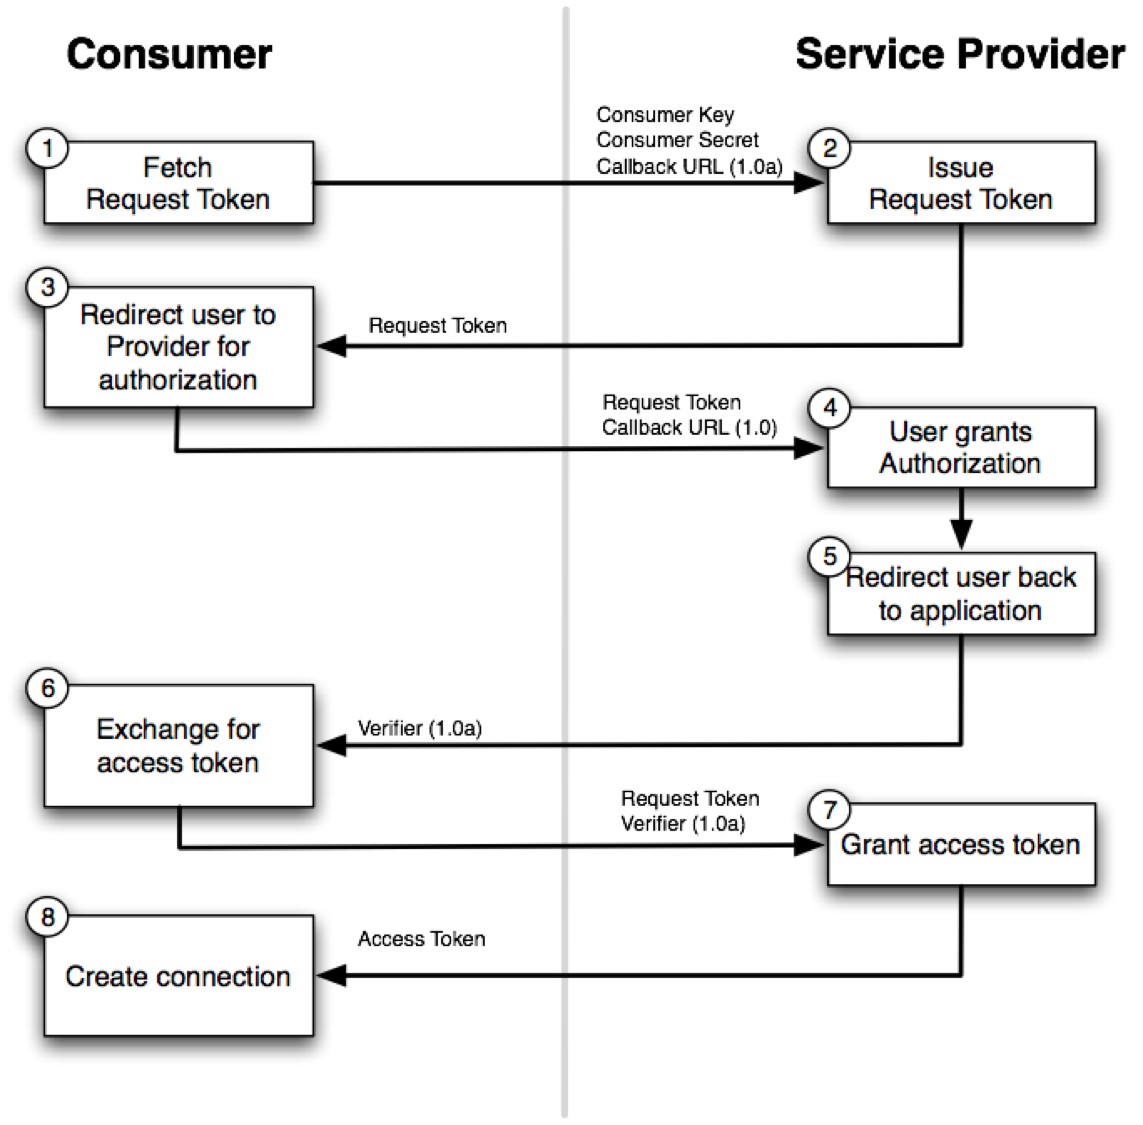
\includegraphics[width=4.5in]{Oauth1a.png}
  		   \caption{Funcionamiento de Oauth1a}
  		   \label{img:oauth1a}
\end{figure}








% Optional in PFCs
%
\chapter{Pliego de condiciones}
\label{cha:pliego-de-condiciones}

Blah, blah, blah.

%%% Local Variables:
%%% TeX-master: "../book"
%%% End:


%Obligatorio en TFGs
\chapter{Conclusiones y futuras líneas de trabajo}
\label{cha:conclusiones y futuras lineas de trabajo}

%
% Fin de la seccion de capitulos
%%%%%%%%%%%%%%%%%%%%%%%%%%%%%%%%%%%%%%%%%%%%%%%%%%%%%%%%%%%%%%%%%%%%%%%%%%%
%%%%%%%%%%%%%%%%%%%%%%%%%%%%%%%%%%%%%%%%%%%%%%%%%%%%%%%%%%%%%%%%%%%%%%%%%%%
%%%%%%%%%%%%%%%%%%%%%%%%%%%%%%%%%%%%%%%%%%%%%%%%%%%%%%%%%%%%%%%%%%%%%%%%%%%


%%%%%%%%%%%%%%%%%%%%%%%%%%%%%%%%%%%%%%%%%%%%%%%%%%%%%%%%%%%%%%%%%%%%%%%%%%%
%
% Generic template for TFC/TFM/TFG/Tesis
%
% $Id: bibliography.tex,v 1.9 2015/06/05 00:10:32 macias Exp $
%
% By:
%  + Javier Macías-Guarasa. 
%    Departamento de Electrónica
%    Universidad de Alcalá
%  + Roberto Barra-Chicote. 
%    Departamento de Ingeniería Electrónica
%    Universidad Politécnica de Madrid   
% 
% Based on original sources by Roberto Barra, Manuel Ocaña, Jesús Nuevo,
% Pedro Revenga, Fernando Herranz and Noelia Hernández. Thanks a lot to
% all of them, and to the many anonymous contributors found (thanks to
% google) that provided help in setting all this up.
%
% See also the additionalContributors.txt file to check the name of
% additional contributors to this work.
%
% If you think you can add pieces of relevant/useful examples,
% improvements, please contact us at (macias@depeca.uah.es)
%
% You can freely use this template and please contribute with
% comments or suggestions!!!
%
%%%%%%%%%%%%%%%%%%%%%%%%%%%%%%%%%%%%%%%%%%%%%%%%%%%%%%%%%%%%%%%%%%%%%%%%%%%

%\bibliographystyle{plainnat}
%\bibliographystyle{dinat}
%\bibliographystyle{unsrt}
\bibliographystyle{IEEEtran}

% The following is overly complicated because I was not able to do so in
% another way. The problem is the bibliography command being "called"
% from both the root and anteproyecto directories...
%
% Here define as many bibfiles as needed
\newcommand{\mybibfileOne}{biblio/biblio.bib}
%\newcommand{\mybibfileTwo}{biblio/biblio2.bib}
%...
%\newcommand{\mybibfileN}{biblio/biblioN}

% This is for a single bib file
\newcommand{\mybibfiles}{\myreferencespath\mybibfileOne}
% but do this for multiple files
%\newcommand{\mybibfiles}{\myreferencespath\mybibfile1,\myreferencespath\mybibfile2,...,\myreferencespath\mybibfileN}

% Do not touch this
\inputencoding{latin1}
\bibliography{\mybibfiles}
\inputencoding{utf8}

%%% Local Variables:
%%% TeX-master: "../book"
%%% coding: utf-8
%%% End:


 % Bibliografia


%%%%%%%%%%%%%%%%%%%%%%%%%%%%%%%%%%%%%%%%%%%%%%%%%%%%%%%%%%%%%%%%%%%%%%%%%%%
% Comienzo de apendices
%                                 

\begin{appendices}
  
\chapter{Funciones implementadas}
\label{cha:funciones}

\section{Función de extracción de Tweets}
\label{sec:funcion-extraccion}

\begin{codefloat}
\inputencoding{latin1}
\lstinputlisting[style=CppExample]{appendix/function.c}
\inputencoding{utf8}
\caption{Extracción de Tweets empleando una funcion en R}
\label{cod:extraccion}
\end{codefloat}

El objetivo fundamental de esta función es extraer los tweets publicados por un usuario y almacenarlos 
en un archivo csv. En caso de que exista un archivo con el mismo nombre, se lee y se concatena el 
nuevo contenido con el antiguo. Los argumentos de entrada, son los siguientes:

\begin{enumerate}

\item usuario: reprsenta el identificador del usuario de Twitter.
\item maxtweets: cantidad de tweets que se van a recuperar.
\item archivoSalida: nombre del fichero de salida.

\end{enumerate}

Se debe tener cuidado de no recuperar tweets repetidos, para ello se ha creado una variable que almacena 
el id del ultimo tweet. Con esto cada vez que se quieran recuperar nuevos tweets, se aumentará en 
uno dicha variable y se procederá como hasta ahora.

%%% Local Variables:
%%% TeX-master: "../book"
%%% End:



\end{appendices}

%
% Fin de apendices
%%%%%%%%%%%%%%%%%%%%%%%%%%%%%%%%%%%%%%%%%%%%%%%%%%%%%%%%%%%%%%%%%%%%%%%%%%%

\backmatter

%%%%%%%%%%%%%%%%%%%%%%%%%%%%%%%%%%%%%%%%%%%%%%%%%%%%%%%%%%%%%%%%%%%%%%%%%%%
%
% Generic template for TFC/TFM/TFG/Tesis
%
% $Id: backpage.tex,v 1.6 2018/12/12 15:29:21 macias Exp $
%
% By:
%  + Javier Macías-Guarasa. 
%    Departamento de Electrónica
%    Universidad de Alcalá
%  + Roberto Barra-Chicote. 
%    Departamento de Ingeniería Electrónica
%    Universidad Politécnica de Madrid   
% 
% Based on original sources by Roberto Barra, Manuel Ocaña, Jesús Nuevo,
% Pedro Revenga, Fernando Herránz and Noelia Hernández. Thanks a lot to
% all of them, and to the many anonymous contributors found (thanks to
% google) that provided help in setting all this up.
%
% See also the additionalContributors.txt file to check the name of
% additional contributors to this work.
%
% If you think you can add pieces of relevant/useful examples,
% improvements, please contact us at (macias@depeca.uah.es)
%
% You can freely use this template and please contribute with
% comments or suggestions!!!
%
%%%%%%%%%%%%%%%%%%%%%%%%%%%%%%%%%%%%%%%%%%%%%%%%%%%%%%%%%%%%%%%%%%%%%%%%%%%

%%%%%%%%%%%%%%%%%%%%%%%%%%%%%%%%%%%%%%%%%%%%%%%%%%%%%%%%%%%%%%%%%%%%%%%%%%%
% Right now (november 2013), it's only defined for TFGs at UAH
%%%%%%%%%%%%%%%%%%%%%%%%%%%%%%%%%%%%%%%%%%%%%%%%%%%%%%%%%%%%%%%%%%%%%%%%%%%

\ifthenelse{\equal{\mybookworktype}{TFG}}
{
  %%%%%%%%%%%%%%%%%%%%%%%%%%%%%%%%%%%%%%%%%%%%%%%%%%%%%%%%%%%%%%%%%%%%%%%%%%%
%
% Generic template for TFC/TFM/TFG/Tesis
%
% $Id: backpage-tfg-uah.tex,v 1.10 2015/06/05 00:10:33 macias Exp $
%
% By:
%  + Javier Macías-Guarasa. 
%    Departamento de Electrónica
%    Universidad de Alcalá
%  + Roberto Barra-Chicote. 
%    Departamento de Ingeniería Electrónica
%    Universidad Politécnica de Madrid   
% 
% Based on original sources by Roberto Barra, Manuel Ocaña, Jesús Nuevo,
% Pedro Revenga, Fernando Herránz and Noelia Hernández. Thanks a lot to
% all of them, and to the many anonymous contributors found (thanks to
% google) that provided help in setting all this up.
%
% See also the additionalContributors.txt file to check the name of
% additional contributors to this work.
%
% If you think you can add pieces of relevant/useful examples,
% improvements, please contact us at (macias@depeca.uah.es)
%
% You can freely use this template and please contribute with
% comments or suggestions!!!
%
%%%%%%%%%%%%%%%%%%%%%%%%%%%%%%%%%%%%%%%%%%%%%%%%%%%%%%%%%%%%%%%%%%%%%%%%%%%

% This is a trick to avoid the header to be shown. There must be a
% better way...
\chapter*{ }
\thispagestyle{empty}

\cleartoleftpage
\thispagestyle{empty}

% To add background watermark, defined in config/preamble.tex
\BgThispage

% Nice example of tikz
% \begin{tikzpicture}[remember picture,overlay]
%   \node [xshift=1cm,yshift=1cm] at (current page.south west)
%   [text width=7cm,fill=red,red!20,rounded corners,above right]
%   {
%     This is an absolutely positioned text in the
%     lower left corner. No shipout-hackery is used.
%   };
% \end{tikzpicture}

\begin{tikzpicture}[remember picture,overlay]
    \node[yshift=-5cm] at (current page.north west)
      {
        \begin{tikzpicture}[remember picture, overlay]
          \draw[fill=headingPortadaTFG,headingPortadaTFG] (0,0) rectangle (\paperwidth,5cm);

          \node [yshift=3cm, xshift=0.5\paperwidth, font=\Huge, text centered, midway] {\color{textoHeadingPortadaTFG}\mybookuniversity};
          \node [yshift=2cm, xshift=0.5\paperwidth, font=\Huge, text centered, midway] {\color{textoHeadingPortadaTFG}\mybookschool};

        \end{tikzpicture}
      };
   \end{tikzpicture}


\large
\vspace{20cm}
\begin{center}
  
  \centerline{
\includegraphics[height=2.5cm]{uah/01_logo-vA_pant293.pdf}}

\end{center}



%%% Local Variables:
%%% TeX-master: "../book"
%%% End:



}
{
\ifthenelse{\equal{\mybookworktype}{TFM}}
{
  %%%%%%%%%%%%%%%%%%%%%%%%%%%%%%%%%%%%%%%%%%%%%%%%%%%%%%%%%%%%%%%%%%%%%%%%%%%
%
% Generic template for TFC/TFM/TFG/Tesis
%
% $Id: backpage-tfg-uah.tex,v 1.10 2015/06/05 00:10:33 macias Exp $
%
% By:
%  + Javier Macías-Guarasa. 
%    Departamento de Electrónica
%    Universidad de Alcalá
%  + Roberto Barra-Chicote. 
%    Departamento de Ingeniería Electrónica
%    Universidad Politécnica de Madrid   
% 
% Based on original sources by Roberto Barra, Manuel Ocaña, Jesús Nuevo,
% Pedro Revenga, Fernando Herránz and Noelia Hernández. Thanks a lot to
% all of them, and to the many anonymous contributors found (thanks to
% google) that provided help in setting all this up.
%
% See also the additionalContributors.txt file to check the name of
% additional contributors to this work.
%
% If you think you can add pieces of relevant/useful examples,
% improvements, please contact us at (macias@depeca.uah.es)
%
% You can freely use this template and please contribute with
% comments or suggestions!!!
%
%%%%%%%%%%%%%%%%%%%%%%%%%%%%%%%%%%%%%%%%%%%%%%%%%%%%%%%%%%%%%%%%%%%%%%%%%%%

% This is a trick to avoid the header to be shown. There must be a
% better way...
\chapter*{ }
\thispagestyle{empty}

\cleartoleftpage
\thispagestyle{empty}

% To add background watermark, defined in config/preamble.tex
\BgThispage

% Nice example of tikz
% \begin{tikzpicture}[remember picture,overlay]
%   \node [xshift=1cm,yshift=1cm] at (current page.south west)
%   [text width=7cm,fill=red,red!20,rounded corners,above right]
%   {
%     This is an absolutely positioned text in the
%     lower left corner. No shipout-hackery is used.
%   };
% \end{tikzpicture}

\begin{tikzpicture}[remember picture,overlay]
    \node[yshift=-5cm] at (current page.north west)
      {
        \begin{tikzpicture}[remember picture, overlay]
          \draw[fill=headingPortadaTFG,headingPortadaTFG] (0,0) rectangle (\paperwidth,5cm);

          \node [yshift=3cm, xshift=0.5\paperwidth, font=\Huge, text centered, midway] {\color{textoHeadingPortadaTFG}\mybookuniversity};
          \node [yshift=2cm, xshift=0.5\paperwidth, font=\Huge, text centered, midway] {\color{textoHeadingPortadaTFG}\mybookschool};

        \end{tikzpicture}
      };
   \end{tikzpicture}


\large
\vspace{20cm}
\begin{center}
  
  \centerline{
\includegraphics[height=2.5cm]{uah/01_logo-vA_pant293.pdf}}

\end{center}



%%% Local Variables:
%%% TeX-master: "../book"
%%% End:



}
{
}
}

%%% Local Variables:
%%% TeX-master: "../book"
%%% End:




\end{document}
